%======================================================================
%	
%	 __  __       _         ______ _ _      
%	|  \/  |     (_)       |  ____(_) |     
%	| \  / | __ _ _ _ __   | |__   _| | ___ 
%	| |\/| |/ _` | | '_ \  |  __| | | |/ _ \
%	| |  | | (_| | | | | | | |    | | |  __/
%	|_|  |_|\__,_|_|_| |_| |_|    |_|_|\___|
%
%----------------------------------------------------------------------
% Descripton : Main File to compose the resulting PDF
%======================================================================
%\pdfobjcompresslevel=0
\pdfminorversion=7
\pdfinclusioncopyfonts=1
\documentclass[
				ngerman             % neue deutsche Rechtschreibung
				,a4paper            % Papiergrösse
				,twoside            % Zweiseitiger Druck (rechts/links)
				% ,10pt             % Schriftgrösse
				,11pt
				% ,12pt
				,pdftex
				%  ,disable         % Todo-Markierungen auschalten
				,notitlepage		% Thanks abstract... preventing it from removing pageNumber
				]{report}

% Bitte die Codierung Ihrer Dateien auswählen:
% \usepackage[latin1]{inputenc}    % Für UNIX mit ISO-LATIN-codierten Dateien
% \usepackage[applemac]{inputenc}  % Für Apple Mac
% \usepackage[ansinew]{inputenc}   % Für Microsoft Windows
\usepackage[utf8]{inputenc}        % UTF-8 codierte Dateien
% Dieses Dokument ist unter Unix erstellt, daher
% wird diese Input-Codierung benutzt.

%————————————————————————————————————————————————————————————————————————————
%					Import aller Konfigurationen
%————————————————————————————————————————————————————————————————————————————
\usepackage{./config/DHBW/bericht}
\usepackage{./config/PaketeProjektarbeit} % <- spezifische Pakete für die Projektarbeit
\usepackage{./config/Pakete}
\usepackage{./config/Befehle}
\usepackage{./config/Layout}
\usepackage{./config/Styles}
%Wenn PDF/A-1B gewünscht .. Achtung am besten nochmal mit veraPDF testen!
\usepackage{./config/PDFStandard}

%————————————————————————————————————————————————————————————————————————————
%					Variablen deklarieren
%————————————————————————————————————————————————————————————————————————————
%======================================================================
%	
%	__      __        _       _     _            
%	\ \    / /       (_)     | |   | |           
%	 \ \  / /_ _ _ __ _  __ _| |__ | | ___ _ __  
%	  \ \/ / _` | '__| |/ _` | '_ \| |/ _ \ '_ \ 
%	   \  / (_| | |  | | (_| | |_) | |  __/ | | |
%	    \/ \__,_|_|  |_|\__,_|_.__/|_|\___|_| |_|
%
%----------------------------------------------------------------------
% Descripton : Variables
%======================================================================

\newboolean{DEBUG}
\newboolean{BERICHTE}
\newboolean{SPERRVERMERK}
\newboolean{CHANGELOG}
\newboolean{VORWORT}
\newboolean{ABSTRACT}
\newboolean{DANKSAGUNG}
\newboolean{WATERMARK}
\newboolean{INDEX}
\newboolean{TRENNSTRICHE}
\newboolean{ERKLAERUNG}
\newboolean{DOKUMENTENVERZEICHNIS}
\newboolean{DATEIVERZEICHNIS}
\newboolean{LITERATURVERWEIS}
\newboolean{DIGITALE-UNTERSCHRIFT}
\newboolean{DIGITAL-SIGN-AREA}
\newboolean{CDBEILAGE}
\newboolean{TODO}

%————————————————————————————————————————————————————————————————————————————
%					Informationen ausfüllen
%————————————————————————————————————————————————————————————————————————————
%======================================================================
%	
%	_____        __                           _   _             
%  |_   _|      / _|                         | | (_)            
%	 | |  _ __ | |_ ___  _ __ _ __ ___   __ _| |_ _  ___  _ __  
%    | | | '_ \|  _/ _ \| '__| '_ ` _ \ / _` | __| |/ _ \| '_ \ 
%	_| |_| | | | || (_) | |  | | | | | | (_| | |_| | (_) | | | |
%  |_____|_| |_|_| \___/|_|  |_| |_| |_|\__,_|\__|_|\___/|_| |_|
%
%----------------------------------------------------------------------
% Descripton : File with all Information about the Document
%======================================================================

% Bei jedem Dokument Anpassen
\newcommand{\Was}{Template}

%%%%%%%%%%%%%%%%%%%%%%%%%%%%%%%%%%%%%%%%%%%%%%%%%%%%%%%%%%%%%%%%%%%%%%%%%%%%%%%%%%%%%

\newcommand{\Titel}{Projektgruppe : TemplateME}
\newcommand{\Autor}{Max Mustermann (\href{mailto:me@somewhere.com}{me@somewhere.com})}
\newcommand{\AutorTwo}{Max Mustermann (\href{mailto:me@somewhere.com}{me@somewhere.com})}
\newcommand{\AutorThree}{Max Mustermann (\href{mailto:me@somewhere.com}{me@somewhere.com})}
\newcommand{\VorlesungsTitel}{Angewandtes Projektmanagement}
\newcommand{\Kursbezeichnung}{tinf17b3}

% Falls es kein Firmenlogo gibt:
\newcommand{\FirmenLogoDeckblatt}{}

\newcommand{\BetreuerDHBW}{Michael Vetter}
\newcommand{\BetreuerStudienarbeit}{XXXXXXXXXXXXXX}

%%%%%%%%%%%%%%%%%%%%%%%%%%%%%%%%%%%%%%%%%%%%%%%%%%%%%%%%%%%%%%%%%%%%%%%%%%%%%%%%%%%%%

\newcommand{\Dauer}{12 Wochen}

% \newcommand{\Abschluss}{Bachelor of Engineering}
\newcommand{\Abschluss}{Bachelor of Science}

%\newcommand{\Studiengang}{Informatik / Informationstechnik}
\newcommand{\Studiengang}{Informatik / Angewandte Informatik}
%======================================================================
%	 _    _                                 __ 
%	| |  | |                               / _|
%	| |__| |_   _ _ __   ___ _ __ _ __ ___| |_ 
%	|  __  | | | | '_ \ / _ \ '__| '__/ _ \  _|
%	| |  | | |_| | |_) |  __/ |  | | |  __/ |  
%	|_|  |_|\__, | .__/ \___|_|  |_|  \___|_|  
%		     __/ | |                           
%		    |___/|_|                           
%
%----------------------------------------------------------------------
% Descripton : Hyperref File for setting PDF Information
%======================================================================

\hypersetup{
	bookmarks=true,
	unicode=false,
	pdftoolbar=true,
	pdfmenubar=true,
	pdffitwindow=false,
	pdfstartview={FitH},
	pdftitle={\Titel},
	pdfauthor={\Autor},
	pdfsubject={\Was},
	pdfcreator={\Autor},
	pdfkeywords={DHBW},
	pdfborderstyle={/S/U/W 1},
	pdfnewwindow=true,
	citebordercolor=LimeGreen,
	filebordercolor=Magenta,
	linkbordercolor=Orange,
	menubordercolor=Orange,
	urlbordercolor=Fuchsia,
	runbordercolor=Orange
}


%————————————————————————————————————————————————————————————————————————————
%					Sonstige Einstellungen
%————————————————————————————————————————————————————————————————————————————
\bibliography{./directories/bibliography}
\loadglsentries{./directories/glossary}
\makeglossaries
\makeindex[columns=1,options={-s ./config/DHBW/bericht.ist}]

%————————————————————————————————————————————————————————————————————————————
%					Einstellungen
%————————————————————————————————————————————————————————————————————————————
% Debug auf true setzen, hierbei wird der Changelog hinzugefügt, und keine Doppelseitenumbrüche gemacht (Zum drucken -> false)
% Bitte zum drucken oben in der Präambel auch auf Doppelseite schalten!
\setboolean{DEBUG}{true}
% Soll der Changelog angezeigt werden ?
\setboolean{CHANGELOG}{true}
% Sollen die TODO's angezeigt werden ?
\setboolean{TODO}{true}
% =================================================================================================
%Digitale Unterschrift auf die Erklärung -> PDF in zfiles/Signaturen/ und dann Signatur.pdf und Ort_Datum.pdf ??
\setboolean{DIGITALE-UNTERSCHRIFT}{true}
%Digitale Unterschriftsfeld auf die Erklärung ??
\setboolean{DIGITAL-SIGN-AREA}{false}
\ifthenelse{\boolean{DIGITAL-SIGN-AREA}}{\setboolean{DIGITALE-UNTERSCHRIFT}{false}}{}
% =================================================================================================
% Soll eine Erklärung eigefügt werden ?
\setboolean{ERKLAERUNG}{true}
%Soll das Abstract eingefügt werden ?
\setboolean{ABSTRACT}{true}
%Soll das Vorwort eingefügt werden ?
\setboolean{VORWORT}{true}
%Soll das Vorwort eingefügt werden ?
\setboolean{DANKSAGUNG}{true}
%Soll ein Sperrvermerk gemacht werden
\setboolean{SPERRVERMERK}{true}
%Literaturverweis auf Speicherung
\setboolean{LITERATURVERWEIS}{true}
% =================================================================================================
% Soll ein Index eingefügt werden ?
\setboolean{INDEX}{true}
%Soll ne Trennlinie im Inhaltsverzeichnis eingefügt werden, vor Verzeichnissen, dem Inhalt und dem Anhang
\setboolean{TRENNSTRICHE}{true}
%Setzt ein Watermark
\setboolean{WATERMARK}{false}
% =================================================================================================
%Dokumentenverzeichnis generieren ?
\setboolean{DOKUMENTENVERZEICHNIS}{true}
%Dateiverzeichnis generieren ?
\setboolean{DATEIVERZEICHNIS}{true}
% Soll auf das Dateiverzeichnis die CD ?
\setboolean{CDBEILAGE}{true}
%Sind Berichte abzugeben ? Automatische einbindung zum Drucken
\setboolean{BERICHTE}{true}

%————————————————————————————————————————————————————————————————————————————
%					Watermark
%————————————————————————————————————————————————————————————————————————————
\ifthenelse{\boolean{WATERMARK}}{\usepackage{draftwatermark}}{}
\ifthenelse{\boolean{WATERMARK}}{\SetWatermarkText{Entwurf}}{}

%————————————————————————————————————————————————————————————————————————————
%					PDF Optionen
%————————————————————————————————————————————————————————————————————————————
%Soll der Changelog angezeigt werden -- Sowieso nur im DEBUG?
\ifthenelse{\boolean{DEBUG}}{}{\setboolean{CHANGELOG}{false}}
%Package um die Referenzen zu checken, einfach im Log nach "refcheck suchen!"
%\usepackage{refcheck}

%————————————————————————————————————————————————————————————————————————————
%									Anfang Dokument
%————————————————————————————————————————————————————————————————————————————
\begin{document}
	% Wer keine Seitenzahlen braucht bis zum TOC einfach das Pagenumbering auf gobble und an der Stelle an der die Seitenzählung beginnen soll roman einfügen
	\pagenumbering{gobble}
	\pagestyle{plain}
	
	%—————————————————————————————————————————————————————————————————————————
	%								Changelog
	%—————————————————————————————————————————————————————————————————————————
	\ifthenelse{\boolean{CHANGELOG}}{
		%======================================================================
%	
%	  _____ _                            _             
%	 / ____| |                          | |            
%	| |    | |__   __ _ _ __   __ _  ___| | ___   __ _ 
%	| |    | '_ \ / _` | '_ \ / _` |/ _ \ |/ _ \ / _` |
%	| |____| | | | (_| | | | | (_| |  __/ | (_) | (_| |
%	 \_____|_| |_|\__,_|_| |_|\__, |\___|_|\___/ \__, |
%						       __/ |              __/ |
%							  |___/              |___/ 
%
%----------------------------------------------------------------------
% Descripton : Changelog
%======================================================================

\chapter*{Änderungen}

\begin{description}
	\item[2022/02/03 - NH] Moved appendix into Pages
	\item[2022/02/03 - NH] Major Structure Refactoring - added IMRAD Schema
	\item[2022/01/17 - NH] Code-Refactoring + Fix für TODONotes + Mehr Output-Streams hinzugefügt im 
							Package
	\item[2022/01/17 - NH] Verzeichnisstruktur angepasst + Kleine Fixes
	\item[2022/01/17 - NH] Bugfix für den Trennstrich
	\item[2021/09/14 - NH] Anpassung der Seitennummern + Korrektur des Dokumentenverzeichnis
	\item[2021/09/01 - NH] Digitale Unterschrift nun möglich .. ob die DHBW das akzeptiert :-/ \\
						   Feld + Boolean für Digital Signing von Adobe eingefügt!
	\item[2021/08/23 - NH] Dokumentenverzeichnis, sowie Dateiverzeichnis hinzugefügt!
	\item[2021/08/18 - NH] PDF/A-1B Standart wird unterstützt .... JUHUUUU
	\item[2021/08/17 - NH] Fixed various Bugs with Booleans + Added own Bibliography for the Presentation!
	\item[2021/08/12 - NH] Refcheck Package eingefügt, um falsche Referenzen einfacher zu finden
	\item[2021/08/03 - NH] Hyperlinks gefixt, und Inhaltsseite eingefügt
	\item[2021/07/23 - NH] Verschiedene Formatierungen gefixt und Index eingefügt
	\item[2021/07/19 - NH] Befehl für Boxshadows eingefügt
	\item[2021/03/10 - NH] Watermark eingefügt
	\item[2020/03/13 - JV] Tippfehler korrigiert\\
	                  aktuelle Formulierungen aus der Prüfungsordnung Technik übernommen\\
	                  Formatdatei erklärt
	\item[2017/10/06 - JV] Anpassung an neuer Versionen diverse Pakete.
	\item[2016/03/16 - JV] Auf UTF-8 umgestellt, Indices.
	\item[2010/04/12 - JV] ToDo-Markierungen mit dem \verb+\todo+-Kommando.
	\item[2010/01/27 - JV] Anhang (\texttt{appendix}), Selbständigkeits-Erklärung, \texttt{framed}-Paket.
	\item[2010/01/21 - JV] Abkürzungen (\texttt{acronym}), \texttt{table} und \texttt{tabular} benutzt,
	     unübliche Pakete beigelegt.
	\item[2010/01/18 - JV] Code-Listings (\texttt{listings}), Literaturreferenzen \texttt{biblatex})
	\item[2010/01/11 - JV] Initiale Version.
\end{description}

		\clearpage
	}{}
	
	%—————————————————————————————————————————————————————————————————————————
	%								TODOS
	%—————————————————————————————————————————————————————————————————————————
	\ifthenelse{\boolean{TODO}}{
		\phantomsection
		\addcontentsline{toc}{chapter}{Liste der ToDo's}
		\listoftodos[Liste der ToDo's]
		\clearpage
		\ifthenelse{\boolean{TRENNSTRICHE}}{\addtocontents{toc}{\protect\mbox{}\protect\hrulefill\par}}{}
	}{}
	
	%—————————————————————————————————————————————————————————————————————————
	%								Deckseite
	%—————————————————————————————————————————————————————————————————————————
	\begin{titlepage}
		%%%%%%%%%%%%%%%%%%%%%%%%%%%%%%%%%%%%%%%%%%%%%%%%%%%%%%%%%%%%%%%%%%%%%%%%%%%%%%%
%% Descr:       Vorlage für Berichte der DHBW-Karlsruhe, Titlepage
%% Author:      Prof. Dr. Jürgen Vollmer, vollmer@dhbw-karlsruhe.de
%% $Id: erklaerung.tex,v 1.11 2020/03/13 14:24:42 vollmer Exp $
%% -*- coding: utf-8 -*-
%%%%%%%%%%%%%%%%%%%%%%%%%%%%%%%%%%%%%%%%%%%%%%%%%%%%%%%%%%%%%%%%%%%%%%%%%%%%%%%

\begin{center}
	\vspace*{-2cm}
	\FirmenLogoDeckblatt\hfill
\includegraphics[width=4cm]{./config/DHBW/dhbw-logo.png}\\[2cm]
	{\Huge \Titel}\\[1cm]
	{\Huge\scshape \Was}\\[1cm]
	{\large für die Prüfung zum}\\[0.5cm]
	{\Large \Abschluss}\\[0.5cm]
	{\large des Studienganges \Studiengang}\\[0.5cm]
	{\large an der}\\[0.5cm]
	{\large Dualen Hochschule Baden-Württemberg Karlsruhe}\\[0.5cm]
	{\large von}\\[0.5cm]
	{\large\bfseries \Autor}\\[1cm]
	{\large Abgabedatum \AbgabeDatum}
	\vfill
\end{center}
\begin{tabular}{l@{\hspace{2cm}}l}
	Bearbeitungszeitraum	         & \Dauer 			\\
	Matrikelnummer	                 & \MatrikelNummer		\\
	Kurs			         & \Kursbezeichnung		\\
	Ausbildungsfirma	         & \FirmenName			\\
	& \FirmenStadt			\\
	Betreuer der Ausbildungsfirma	 & \BetreuerFirma		\\
	Gutachter der Studienakademie	 & \BetreuerDHBW		\\
\end{tabular}
	\end{titlepage}
	
	% Ab hier beginnt die Seitenzählung für den Prefix in kleinen römischen Zahlen
	% Erste Seite nach der Titelseite
	\pagenumbering{roman}
	\setcounter{page}{2}
	\ifthenelse{\boolean{DEBUG}}{}{\cleardoublepage}
	
	
	
	%—————————————————————————————————————————————————————————————————————————
	%								Erklärung
	%—————————————————————————————————————————————————————————————————————————
	\ifthenelse{\boolean{ERKLAERUNG}}{
		\phantomsection
		%%%%%%%%%%%%%%%%%%%%%%%%%%%%%%%%%%%%%%%%%%%%%%%%%%%%%%%%%%%%%%%%%%%%%%%%%%%%%%%
%% Descr:       Vorlage für Berichte der DHBW-Karlsruhe, Erklärung
%% Author:      Prof. Dr. Jürgen Vollmer, vollmer@dhbw-karlsruhe.de
%% $Id: erklaerung.tex,v 1.11 2020/03/13 14:24:42 vollmer Exp $
%% -*- coding: utf-8 -*-
%%%%%%%%%%%%%%%%%%%%%%%%%%%%%%%%%%%%%%%%%%%%%%%%%%%%%%%%%%%%%%%%%%%%%%%%%%%%%%%

% In Bachelorarbeiten muss eine schriftliche Erklärung abgegeben werden.
% Hierin bestätigen die Studierenden, dass die Bachelorarbeit, etc.
% selbständig verfasst und sämtliche Quellen und Hilfsmittel angegeben sind. Diese Erklärung
% bildet das zweite Blatt der Arbeit. Der Text dieser Erklärung muss auf einer separaten Seite
% wie unten angegeben lauten.

\newpage
\thispagestyle{empty}
\begin{framed}
\begin{center}
\Large\bfseries Erklärung
\end{center}
\medskip
\noindent
% siehe §5(3) der \enquote{Studien- und Prüfungsordnung DHBW Technik} vom 29.\,9.\,2017 und Anhang 1.1.13
Ich versichere hiermit, dass ich meine \Was \ mit dem Thema:
\enquote{\Titel}
selbstständig verfasst und keine anderen als die angegebenen Quellen und Hilfsmittel benutzt habe. Ich versichere zudem, dass die eingereichte elektronische Fassung mit der gedruckten Fassung übereinstimmt. \\
\vspace{3cm} \\
\ifthenelse{\boolean{DIGITALE-UNTERSCHRIFT}}{
\includegraphics[height=1.5\baselineskip]{./zfiles/Signaturen/Ort_Datum} \hfill 
\includegraphics[height=2\baselineskip]{./zfiles/Signaturen/Signatur} \hspace{0.1cm} \vspace{-0.5cm} \\}{}
\ifthenelse{\boolean{DIGITAL-SIGN-AREA}}{\sigField{Digitale Signatur}{14cm}{2cm}}{}
\ifthenelse{\boolean{DIGITAL-SIGN-AREA}}{\underline{\hspace{14cm}} \\ \hspace{4cm} Digitale Unterschrift}{\underline{\hspace{6cm}}\hfill\underline{\hspace{6cm}} \\ Ort~~~~~~~~~~~~~Datum \hfill Unterschrift\hspace{4cm}}
\end{framed}

%%%%%%%%%%%%%%%%%%%%%%%%%%%%%%%%%%%%%%%%%%%%%%%%%%%%%%%%%%%%%%%%%%%%%%%%%%%%%%%
\endinput
%%%%%%%%%%%%%%%%%%%%%%%%%%%%%%%%%%%%%%%%%%%%%%%%%%%%%%%%%%%%%%%%%%%%%%%%%%%%%%%

		\addcontentsline{toc}{chapter}{Erklärung}
	}{}
	\ifthenelse{\boolean{SPERRVERMERK}}{%%%%%%%%%%%%%%%%%%%%%%%%%%%%%%%%%%%%%%%%%%%%%%%%%%%%%%%%%%%%%%%%%%%%%%%%%%%%%%%
%% Descr:       Vorlage für Berichte der DHBW-Karlsruhe, Sperrvermerk
%% Author:      Prof. Dr. Jürgen Vollmer, vollmer@dhbw-karlsruhe.de
%% $Id: sperrvermerk.tex,v 1.11 2020/03/13 14:24:42 vollmer Exp $
%% -*- coding: utf-8 -*-
%%%%%%%%%%%%%%%%%%%%%%%%%%%%%%%%%%%%%%%%%%%%%%%%%%%%%%%%%%%%%%%%%%%%%%%%%%%%%%%

\vfill
\begin{framed}
\begin{center}
\Large\bfseries Sperrvermerk
\end{center}
\medskip
\noindent
%%%%%%%%%%%%%%%%%%%%%%%%%%%%%%%%%%%%%%%%%%%%%%%%%%%%%%%%%%%%%%%%%%%%%%%%%%%%%%%
%% Descr:       Vorlage für Berichte der DHBW-Karlsruhe, Sperrvermerk
%% Author:      Prof. Dr. Jürgen Vollmer, vollmer@dhbw-karlsruhe.de
%% $Id: sperrvermerk.tex,v 1.11 2020/03/13 14:24:42 vollmer Exp $
%% -*- coding: utf-8 -*-
%%%%%%%%%%%%%%%%%%%%%%%%%%%%%%%%%%%%%%%%%%%%%%%%%%%%%%%%%%%%%%%%%%%%%%%%%%%%%%%
Der Inhalt dieser Arbeit darf weder als Ganzes noch in Auszügen Personen
außerhalb des Prüfungsprozesses und des Evaluationsverfahrens zugänglich gemacht
werden, sofern keine anderslautende Genehmigung vom Dualen Partner vorliegt.
\end{framed}}{}
	\ifthenelse{\boolean{DEBUG}}{}{\cleardoublepage}
	
	%—————————————————————————————————————————————————————————————————————————
	%								Abstract
	%—————————————————————————————————————————————————————————————————————————
	\ifthenelse{\boolean{ABSTRACT}}{
		\phantomsection
		%%%%%%%%%%%%%%%%%%%%%%%%%%%%%%%%%%%%%%%%%%%%%%%%%%%%%%%%%%%%%%%%%%%%%%%%%%%%%%%
%% Descr:       Vorlage für Berichte der DHBW-Karlsruhe, Abstract
%% Author:      Prof. Dr. Jürgen Vollmer, vollmer@dhbw-karlsruhe.de
%% $Id: abstract.tex,v 1.11 2020/03/13 14:24:42 vollmer Exp $
%% -*- coding: utf-8 -*-
%%%%%%%%%%%%%%%%%%%%%%%%%%%%%%%%%%%%%%%%%%%%%%%%%%%%%%%%%%%%%%%%%%%%%%%%%%%%%%%

\vspace*{5cm}
%\vspace*{\fill}

\begingroup
	\centering
	\begin{abstract}
		\addcontentsline{toc}{chapter}{Zusammenfassung}
		Dieses \LaTeX-Dokument kann als Vorlage für einen Praxis- oder Projektbericht, eine Studien- oder Bachelorarbeit dienen.
		Zusammengestellt von Prof.\,Dr.\,Jürgen Vollmer \email{juergen.vollmer@dhbw-karlsruhe.de}
		\url{https://www.karlsruhe.dhbw.de} modifiziert von Nico Holzhäuser \email{nico.holzhaeuser@abilis.de} \url{https://abilis.de}. \\
		Die jeweils aktuellste Version dieses \LaTeX-Paketes ist immer
		auf der \emph{FAQ-Seite} des Studiengangs Informatik zu finden:
		\url{https://www.karlsruhe.dhbw.de/inf/studienverlauf-organisatorisches.html} $\to$ \emph{Formulare und Vorlagen}.
		\centering Stand \verb+$Date: 2020/09/17 15:07:45 $+
		\centering Stand DHBW \verb+$Date: 2020/03/13 15:07:45 $+
	\end{abstract}
\endgroup

\vspace*{\fill}
	}{}
	\ifthenelse{\boolean{DEBUG}}{}{\cleardoublepage}
	
	
	%—————————————————————————————————————————————————————————————————————————
	%								Vorwort
	%—————————————————————————————————————————————————————————————————————————
	\ifthenelse{\boolean{VORWORT}}{
		\phantomsection
		\addcontentsline{toc}{chapter}{Vorwort}
		%%%%%%%%%%%%%%%%%%%%%%%%%%%%%%%%%%%%%%%%%%%%%%%%%%%%%%%%%%%%%%%%%%%%%%%%%%%%%%%
%% Descr:       Vorlage für Berichte der DHBW-Karlsruhe, Abstract
%% Author:      Prof. Dr. Jürgen Vollmer, vollmer@dhbw-karlsruhe.de
%% $Id: abstract.tex,v 1.11 2020/03/13 14:24:42 vollmer Exp $
%% -*- coding: utf-8 -*-
%%%%%%%%%%%%%%%%%%%%%%%%%%%%%%%%%%%%%%%%%%%%%%%%%%%%%%%%%%%%%%%%%%%%%%%%%%%%%%%

\chapter*{Vorwort}
Lore ipsum

	}{}
	\ifthenelse{\boolean{DEBUG}}{}{\cleardoublepage}
	
	%—————————————————————————————————————————————————————————————————————————
	%								Danksagung
	%—————————————————————————————————————————————————————————————————————————
	\ifthenelse{\boolean{DANKSAGUNG}}{
		\phantomsection
		%%%%%%%%%%%%%%%%%%%%%%%%%%%%%%%%%%%%%%%%%%%%%%%%%%%%%%%%%%%%%%%%%%%%%%%%%%%%%%%
%% Descr:       Vorlage für Berichte der DHBW-Karlsruhe, Abstract
%% Author:      Prof. Dr. Jürgen Vollmer, vollmer@dhbw-karlsruhe.de
%% $Id: abstract.tex,v 1.11 2020/03/13 14:24:42 vollmer Exp $
%% -*- coding: utf-8 -*-
%%%%%%%%%%%%%%%%%%%%%%%%%%%%%%%%%%%%%%%%%%%%%%%%%%%%%%%%%%%%%%%%%%%%%%%%%%%%%%%

\chapter*{Danksagung}
Ich danke allen <3
	}{}
	\ifthenelse{\boolean{DEBUG}}{}{\cleardoublepage}
	
	\ifthenelse{\boolean{TRENNSTRICHE}}{\addtocontents{toc}{\protect\mbox{}\protect\hrulefill\par}}{}
	
	%—————————————————————————————————————————————————————————————————————————
	%							Inhaltsverzeichnis
	%—————————————————————————————————————————————————————————————————————————
	\setcounter{tocdepth}{1}% Allow only \chapter in ToC
	\ifthenelse{\boolean{DEBUG}}{}{\cleardoublepage}
	
	\phantomsection
	\addcontentsline{toc}{chapter}{Inhaltsverzeichnis}
	\tableofcontents           % Inhaltsverzeichnis hier ausgeben
	\ifthenelse{\boolean{DEBUG}}{\newpage}{\cleardoublepage}
	
	\phantomsection
	\listoffigures             % Liste der Abbildungen
	\addcontentsline{toc}{chapter}{Abbildungsverzeichnis}
	\ifthenelse{\boolean{DEBUG}}{\newpage}{\cleardoublepage}
	
	\phantomsection
	\listoftables              % Liste der Tabellen
	\addcontentsline{toc}{chapter}{Tabellenverzeichnis}
	\ifthenelse{\boolean{DEBUG}}{\newpage}{\cleardoublepage}
	
	\phantomsection
	\lstlistoflistings         % Liste der Listings
	\addcontentsline{toc}{chapter}{Codeverzeichnis}
	\ifthenelse{\boolean{DEBUG}}{\newpage}{\cleardoublepage}
	
	\phantomsection
	\addcontentsline{toc}{chapter}{Formelverzeichnis}
	\listofequations   % Liste der Formeln
	\ifthenelse{\boolean{DEBUG}}{\newpage}{\cleardoublepage}
	
	\phantomsection
	%======================================================================
%                                              
%	    /\                                        
%	   /  \   ___ _ __ ___  _ __  _   _ _ __ ___  
%	  / /\ \ / __| '__/ _ \| '_ \| | | | '_ ` _ \ 
%	 / ____ \ (__| | | (_) | | | | |_| | | | | | |
%	/_/    \_\___|_|  \___/|_| |_|\__, |_| |_| |_|
% 	                              __/ |          
%	                              |___/             
%
%----------------------------------------------------------------------
% Author : Nico Holzhäuser
% Descripton : Cover Page
%======================================================================

\chapter*{Abkürzungsverzeichnis} % chapter*{..} --> keine Nummer, kein "Kapitel"
						         % Nicht ins Inhaltsverzeichnis
\addcontentsline{toc}{chapter}{Abkürzungsverzeichnis}   % Damit das doch ins Inhaltsverzeichnis kommt

% Hier werden die Abkürzungen definiert
% 1-10 nur damit der Abstand default auf diese Länge gesetzt wird
\begin{acronym}[12345678910]
  	%\acro{Name}{Darstellung der Abkürzung}{Langform der Abkürzung}
	\acro{WWW}[WWW]{World Wide Web}
	\acro{Abk}[Abk.]{Abkürzung}
	\acro{H2O}[\ensuremath{H_2O}]{Di-Hydrogen-Monoxid}
	\acro{DHBW}[DHBW]{Duale Hochschule Baden-Württemberg}


	% Folgendes benutzen, wenn der Plural einer Abk. benöigt wird
	% \newacroplural{Name}{Darstellung der Abkürzung}{Langform der Abkürzung}
	\newacroplural{Abk}[Abk-en]{Abkürzungen}

	% Wenn neicht benutzt, erscheint diese Abk. nicht in der Liste
	\acro{NUA}[]{Not Used Acronym}
	
\end{acronym}
 %Acronyms
	\ifthenelse{\boolean{DEBUG}}{\newpage}{\cleardoublepage}
	
	\phantomsection
	%\addcontentsline{toc}{chapter}{Glossar} %Glossar
	% Wenn Glossar nicht erstellt wird -> In den Projektarbeitspaketen automake=true setzen ....
	\printglossaries
	
	\ifthenelse{\boolean{TRENNSTRICHE}}{\addtocontents{toc}{\protect\mbox{}\protect\hrulefill\par}}{}
	
	\ifthenelse{\boolean{DEBUG}}{\newpage}{\cleardoublepage}
	
	%—————————————————————————————————————————————————————————————————————————
	%								Inhalt
	%—————————————————————————————————————————————————————————————————————————
	%Hauptteil normale arabische Zählung, beginnend bei 1 und alten Pagestyle wiederherstellen!
	\pagenumbering{arabic} 
	\setcounter{page}{1}
	\pagestyle{headings} %<- Pagestyle reset 
	
	%—————————————————————————————————————————————————————————————————————————
	%								IMRAD Schema
	%	https://tu-dresden.de/ing/informatik/smt/cgv/ressourcen/dateien/materialien/howto-abschlussarbeit.pdf?lang=de
	%
	%	Kapitel 1 Einleitung Hier die Problemstellung im Anwendungskontext motivieren, die 
	%	Aufgabenstellung mit eigenen Worten wiedergeben und einen Überblick über die Arbeit 
	%	geben.
	%% !TeX spellcheck = de_DE
%%%%%%%%%%%%%%%%%%%%%%%%%%%%%%%%%%%%%%%%%%%%%%%%%%%%%%%%%%%%%%%%%%%%%%%%%%%%%%%%%%%%%%%%%
%  ______ _       _      _ _                     
% |  ____(_)     | |    (_) |                    
% | |__   _ _ __ | | ___ _| |_ _   _ _ __   __ _ 
% |  __| | | '_ \| |/ _ \ | __| | | | '_ \ / _` |
% | |____| | | | | |  __/ | |_| |_| | | | | (_| |
% |______|_|_| |_|_|\___|_|\__|\__,_|_| |_|\__, |
%										    __/ |
%										   |___/ 
%%%%%%%%%%%%%%%%%%%%%%%%%%%%%%%%%%%%%%%%%%%%%%%%%%%%%%%%%%%%%%%%%%%%%%%%%%%%%%%%%%%%%%%%%
% 	Ganz am Anfang der schriftlichen Ausarbeitung soll die Einleitung eine griffige Motivation für die Aufgabe geben 
%	und elegant in das Thema einführen. Hier wird die Problemstellung im Kontext einer Anwendung dargestellt und der 
%	Inhalt der Arbeit kurz vorweggenommen. Welches Problem wurde gelöst, warum ist das relevant? Wie ist die 
%	Vorgehensweise? Was wurde thematisch eingegrenzt, was wurde ausgegrenzt? Wichtig ist es, den eigenen Beitrag in 
%	wenigen prägnanten Sätzen herauszuarbeiten. (Das Fazit soll sich zum Schluss auf diese Beiträge beziehen, um der %
%	Arbeit eine erzählerische Klammer zu geben.) Die Einleitung endet mit einem Überblick über die Arbeit – hierbei 
%	werden die Inhalte der einzelnen Kapitel knapp umschrieben (vermeiden Sie hier triviale Aussagen wie "Im 
%	Ergebniskapitel 7 werden die Ergebnisse präsentiert.") Tipp: Vermeiden Sie Standard-Intros wie „XY ist in der 
%	Computergraphik ein wichtiges Anwendungsfeld“ oder „In der Computergraphik ist XY nicht mehr wegzudenken“.
%%%%%%%%%%%%%%%%%%%%%%%%%%%%%%%%%%%%%%%%%%%%%%%%%%%%%%%%%%%%%%%%%%%%%%%%%%%%%%%%%%%%%%%%%
\chapter{Einleitung} \label{1.einleitung}
	
	\section{Placeholder}
		\lipsum \gls{real number} \index{TEST}	\ifthenelse{\boolean{DEBUG}}{}{\cleardoublepage}
	%	Kapitel 2 Verwandte Arbeiten Aufzeigen, wer sich bereits mit dem Thema oder 
	%	ähnlichen verwandten Themen auseinandergesetzt hat, welche Lösungswege beschrieben %	wurden und was die Verbindung der jeweiligen zur eigenen Arbeit ist.
	%% !TeX spellcheck = de_DE
%%%%%%%%%%%%%%%%%%%%%%%%%%%%%%%%%%%%%%%%%%%%%%%%%%%%%%%%%%%%%%%%%%%%%%%%%%%%%%%%%%%%%%%%%
%										    _ _       
%										   | | |      
%	__   _____ _ ____      ____ _ _ __   __| | |_ ___ 
%	\ \ / / _ \ '__\ \ /\ / / _` | '_ \ / _` | __/ _ \
%	 \ V /  __/ |   \ V  V / (_| | | | | (_| | ||  __/
%	  \_/ \___|_|    \_/\_/ \__,_|_| |_|\__,_|\__\___|
%
%				   _          _ _             
%		/\        | |        (_) |            
%	   /  \   _ __| |__   ___ _| |_ ___ _ __  
%	  / /\ \ | '__| '_ \ / _ \ | __/ _ \ '_ \ 
%	 / ____ \| |  | |_) |  __/ | ||  __/ | | |
%	/_/    \_\_|  |_.__/ \___|_|\__\___|_| |_|
%%%%%%%%%%%%%%%%%%%%%%%%%%%%%%%%%%%%%%%%%%%%%%%%%%%%%%%%%%%%%%%%%%%%%%%%%%%%%%%%%%%%%%%%%
%	Es soll aufgezeigt werden, wer sich bereits mit dem Thema oder ähnlichen verwandten Themen auseinandergesetzt hat,
%	welche Lösungswege beschrieben wurden und was die Verbindung der jeweiligen Arbeit zur eigenen ist. Beachten Sie
%	die “4 W” als Gedankenstütze: 
%		Welches Problem wurde angegangen? 
%		Wie wurde das Problem gelöst? 
%		Was hat es gebracht? 
%		Wie steht es in Verbindung mit der eigenen Arbeit? 
%	In diesem Kapitel ist es besonders schwierig, einen roten Faden zu erzeugen und zu verhindern, dass der Text zu 
%	einer Paperauflistung verkommt. Es bieten sich Strategien an, die auch kombinierbar sind: Chronologisch oder 
%	aspektorientiert. Bei der chronologischen Auflistung beschreibt man verwandte Arbeiten zeitlich sortiert und gibt 
%	dadurch einen historischen Abriss über die Lösungsansätze des betrachteten Problems. Typischerweise beschreibt 
%	man die zeitlich erste Quelle genauer, sowie die zeitlich näher folgenden Quellen. Anschließend kann man etwas 
%	springen und sich auf Meilensteine konzentrieren. Schließlich sollte der aktuelle Stand wieder genauer betrachtet 
%	werden. Die zweite Strategie, aspektorientiertes Zitieren, sieht eine Unterteilung der Paper in Aspekte des 
%	eigenen Problems vor. Geht es zum Beispiel um Volume-Rendering mit globaler Beleuchtung, sollten Papers zum 
%	Volume-Rendering allgemein, dann Quellen zu erweiterten Methoden und schließlich Papers zur Integration von 
%	globaler Beleuchtung nacheinander (eventuell sogar in getrennten Abschnitten) vorgestellt werden.
%%%%%%%%%%%%%%%%%%%%%%%%%%%%%%%%%%%%%%%%%%%%%%%%%%%%%%%%%%%%%%%%%%%%%%%%%%%%%%%%%%%%%%%%%
\chapter{Verwandte Arbeiten} \label{2.verwandteArbeiten}

	\section{Placeholder}
		\lipsum	\ifthenelse{\boolean{DEBUG}}{}{\cleardoublepage}
	%	Kapitel 3 Grundlagen Vorstellung von mathematischem, technischem, algorithmischem %	
	%	oder anderem Grundlagenwissen, um die Arbeit zu verstehen.
	%% !TeX spellcheck = de_DE
%%%%%%%%%%%%%%%%%%%%%%%%%%%%%%%%%%%%%%%%%%%%%%%%%%%%%%%%%%%%%%%%%%%%%%%%%%%%%%%%%%%%%%%%%
%   _____                      _ _                        
%  / ____|                    | | |                       
% | |  __ _ __ _   _ _ __   __| | | __ _  __ _  ___ _ __  
% | | |_ | '__| | | | '_ \ / _` | |/ _` |/ _` |/ _ \ '_ \ 
% | |__| | |  | |_| | | | | (_| | | (_| | (_| |  __/ | | |
%  \_____|_|   \__,_|_| |_|\__,_|_|\__,_|\__, |\___|_| |_|
% 										  __/ |           
% 										 |___/            
%%%%%%%%%%%%%%%%%%%%%%%%%%%%%%%%%%%%%%%%%%%%%%%%%%%%%%%%%%%%%%%%%%%%%%%%%%%%%%%%%%%%%%%%%
%	Hier soll mathematisches, technisches, algorithmisches und anderes Wissen erklärt werden, aber nur soviel, wie für 
%	das Verständnis der Arbeit gebraucht wird. Als bekanntes Vorwissen kann der eigene Wissensstand vor Antritt der 
%	Arbeit angesehen werden. Weiterführendes Grundlagenwissen oder detaillierte mathematische Herleitungen in den 
%	Anhang verschieben. Die Arbeit ist kein Lehrbuch! Eventuell können hier Erklärungen der verwendeten Fachbegriffe 
%	stehen (oder am Anfang des MethodikKapitels).
%%%%%%%%%%%%%%%%%%%%%%%%%%%%%%%%%%%%%%%%%%%%%%%%%%%%%%%%%%%%%%%%%%%%%%%%%%%%%%%%%%%%%%%%%
\chapter{Theoretische Grundlagen} \label{3.theoretischeGrundlagen}

	\section{Placeholder}
		\lipsum	\ifthenelse{\boolean{DEBUG}}{}{\cleardoublepage}
	%	Kapitel 4ff Methodik und Umsetzung Hauptteil der Arbeit – hier zunächst die 
	%	Konzeption, danach die Realisierung beschreiben.
	%% !TeX spellcheck = de_DE
%%%%%%%%%%%%%%%%%%%%%%%%%%%%%%%%%%%%%%%%%%%%%%%%%%%%%%%%%%%%%%%%%%%%%%%%%%%%%%%%%%%%%%%%%
%	 __  __      _   _               _ _ _    
%	|  \/  |    | | | |             | (_) |   
%	| \  / | ___| |_| |__   ___   __| |_| | __
%	| |\/| |/ _ \ __| '_ \ / _ \ / _` | | |/ /
%	| |  | |  __/ |_| | | | (_) | (_| | |   < 
%	|_|  |_|\___|\__|_| |_|\___/ \__,_|_|_|\_\
%%%%%%%%%%%%%%%%%%%%%%%%%%%%%%%%%%%%%%%%%%%%%%%%%%%%%%%%%%%%%%%%%%%%%%%%%%%%%%%%%%%%%%%%%
%	Hier wird die eigene Arbeit zunächst konzeptuell beschrieben, darunter fällt die Problemanalyse und die 
%	Lösungssuche/-findung. An dieser Stelle soll eine theoretische Auseinandersetzung mit dem Stoff stattfinden – 
%	erklären Sie nicht anhand von konkreten APIs oder Quellcode (Pseudocode hingegen ist erlaubt). Erst danach folgt 
%	die Beschreibung der Realisierung – in den meisten Fällen die Implementierung als Software. Achten Sie hierbei auf 
%	eine übersichtliche und problembezogene Auswahl an Code-Beispielen oder (Teil-)Klassendiagrammen. Detaillierte und 
%	umfassende Darstellungen sollten, wenn überhaupt notwendig, in den Anhang.
%%%%%%%%%%%%%%%%%%%%%%%%%%%%%%%%%%%%%%%%%%%%%%%%%%%%%%%%%%%%%%%%%%%%%%%%%%%%%%%%%%%%%%%%%
\chapter{Methodik} \label{4.methodik}

	\section{Placeholder}
		\lipsum	\ifthenelse{\boolean{DEBUG}}{}{\cleardoublepage}
	%% !TeX spellcheck = de_DE
%%%%%%%%%%%%%%%%%%%%%%%%%%%%%%%%%%%%%%%%%%%%%%%%%%%%%%%%%%%%%%%%%%%%%%%%%%%%%%%%%%%%%%%%%	
%	 _    _                    _                         
%	| |  | |                  | |                        
%	| |  | |_ __ ___  ___  ___| |_ _____   _ _ __   __ _ 
%	| |  | | '_ ` _ \/ __|/ _ \ __|_  / | | | '_ \ / _` |
%	| |__| | | | | | \__ \  __/ |_ / /| |_| | | | | (_| |
%	 \____/|_| |_| |_|___/\___|\__/___|\__,_|_| |_|\__, |
%													__/ |
%												   |___/ 
%%%%%%%%%%%%%%%%%%%%%%%%%%%%%%%%%%%%%%%%%%%%%%%%%%%%%%%%%%%%%%%%%%%%%%%%%%%%%%%%%%%%%%%%%
%	Hier wird die eigene Arbeit zunächst konzeptuell beschrieben, darunter fällt die Problemanalyse und die 
%	Lösungssuche/-findung. An dieser Stelle soll eine theoretische Auseinandersetzung mit dem Stoff stattfinden – 
%	erklären Sie nicht anhand von konkreten APIs oder Quellcode (Pseudocode hingegen ist erlaubt). Erst danach folgt 
%	die Beschreibung der Realisierung – in den meisten Fällen die Implementierung als Software. Achten Sie hierbei auf 
%	eine übersichtliche und problembezogene Auswahl an Code-Beispielen oder (Teil-)Klassendiagrammen. Detaillierte und 
%	umfassende Darstellungen sollten, wenn überhaupt notwendig, in den Anhang.
%%%%%%%%%%%%%%%%%%%%%%%%%%%%%%%%%%%%%%%%%%%%%%%%%%%%%%%%%%%%%%%%%%%%%%%%%%%%%%%%%%%%%%%%%
\chapter{Umsetzung} \label{5.umsetzung}

\section{Placeholder}
\lipsum	\ifthenelse{\boolean{DEBUG}}{}{\cleardoublepage}
	%	Kapitel 4ff +1 Ergebnisse Die Ergebnisse objektiv darstellen und beschreiben, wie 
	%	genau die Ergebnisse erhoben wurden. Auf Besonderheiten aufmerksam machen.
	%% !TeX spellcheck = de_DE
%%%%%%%%%%%%%%%%%%%%%%%%%%%%%%%%%%%%%%%%%%%%%%%%%%%%%%%%%%%%%%%%%%%%%%%%%%%%%%%%%%%%%%%%%		
%	 ______                _           _              
%	|  ____|              | |         (_)             
%	| |__   _ __ __ _  ___| |__  _ __  _ ___ ___  ___ 
%	|  __| | '__/ _` |/ _ \ '_ \| '_ \| / __/ __|/ _ \
%	| |____| | | (_| |  __/ |_) | | | | \__ \__ \  __/
%	|______|_|  \__, |\___|_.__/|_| |_|_|___/___/\___|
%				 __/ |                                
%				|___/                                 
%%%%%%%%%%%%%%%%%%%%%%%%%%%%%%%%%%%%%%%%%%%%%%%%%%%%%%%%%%%%%%%%%%%%%%%%%%%%%%%%%%%%%%%%%
%	Hier erfolgt eine objektive Darstellung der Ergebnisse. Dabei ist eine Unterteilung in quantitative Evaluation 
%	(Erzeugung von Messdaten) und qualitative Evaluation (Umfragen, Expertenfeedback, Beschreibung von Besonderheiten) 
%	sinnvoll. Pro evaluiertem Sachverhalt sollte zunächst das Ergebnis (z.B. als Abbildung oder Tabelle) gezeigt 
%	werden, danach wird es beschrieben und erst anschließend gedeutet. Eine Bewertung findet noch nicht statt.
%%%%%%%%%%%%%%%%%%%%%%%%%%%%%%%%%%%%%%%%%%%%%%%%%%%%%%%%%%%%%%%%%%%%%%%%%%%%%%%%%%%%%%%%%
\chapter{Ergebnisse} \label{6.ergebnisse}

\section{Placeholder}
\lipsum	\ifthenelse{\boolean{DEBUG}}{}{\cleardoublepage}
	%	Kapitel 4ff +2 Diskussion Die umgesetzte Lösung an den Ergebnissen diskutieren. 
	%	Besonderheiten nachvollziehen, erläutern. Darauf aufbauend das Pro und Contra (des 
	%	entwickelten Verfahrens) herausarbeiten. Unter Umständen können die Kapitel 
	%	"Ergebnisse" und "Diskussion" in einem gemeinsamen Kapitel zusammengefasst werden.
	%% !TeX spellcheck = de_DE
%%%%%%%%%%%%%%%%%%%%%%%%%%%%%%%%%%%%%%%%%%%%%%%%%%%%%%%%%%%%%%%%%%%%%%%%%%%%%%%%%%%%%%%%% 
%	 _____  _     _                  _             
%	|  __ \(_)   | |                (_)            
%	| |  | |_ ___| | ___   _ ___ ___ _  ___  _ __  
%	| |  | | / __| |/ / | | / __/ __| |/ _ \| '_ \ 
%	| |__| | \__ \   <| |_| \__ \__ \ | (_) | | | |
%	|_____/|_|___/_|\_\\__,_|___/___/_|\___/|_| |_|
%%%%%%%%%%%%%%%%%%%%%%%%%%%%%%%%%%%%%%%%%%%%%%%%%%%%%%%%%%%%%%%%%%%%%%%%%%%%%%%%%%%%%%%%%
%	Erst im Diskussionsteil sind die Ergebnisse kritisch zu hinterfragen und einzuschätzen. Darauf aufbauend wird das 
%	Pro und Contra (des entwickelten Verfahrens) herausgearbeitet.
%%%%%%%%%%%%%%%%%%%%%%%%%%%%%%%%%%%%%%%%%%%%%%%%%%%%%%%%%%%%%%%%%%%%%%%%%%%%%%%%%%%%%%%%%
\chapter{Diskussion} \label{7.diskussion}

\section{Placeholder}
\lipsum	\ifthenelse{\boolean{DEBUG}}{}{\cleardoublepage}
	%	Kapitel 4ff +3 Zusammenfassung Kurze Zusammenfassung und Bewertung, die 
	%	Ergebnisse/Lösungen werden in einem Fazit kondensiert.
	%% !TeX spellcheck = de_DE
%%%%%%%%%%%%%%%%%%%%%%%%%%%%%%%%%%%%%%%%%%%%%%%%%%%%%%%%%%%%%%%%%%%%%%%%%%%%%%%%%%%%%%%%% 
%	 ______        _ _   
%	|  ____|      (_) |  
%	| |__ __ _ _____| |_ 
%	|  __/ _` |_  / | __|
%	| | | (_| |/ /| | |_ 
%	|_|  \__,_/___|_|\__|
%%%%%%%%%%%%%%%%%%%%%%%%%%%%%%%%%%%%%%%%%%%%%%%%%%%%%%%%%%%%%%%%%%%%%%%%%%%%%%%%%%%%%%%%%
%	Die Arbeit wird kurz zusammengefasst und bewertet, die Ergebnisse/Lösungen in einem Fazit kondensiert (hierbei den 
%	Bogen zu den in der Einleitung aufgeworfenen Problemstellungen spannen). Es kann eine Einschätzung zur allgemeinen 
%	Nützlichkeit der entwickelten Verfahren gegeben werden. 
%		Tipp: Enden Sie mit etwas Positivem! Zeigen Sie im Fazit zunächst die „guten“ Dinge, danach die „schlechten“. 
%		Für letztere merken Sie an, dass sie lösbar sind und dass die entwickelten Verfahren nichtsdestotrotz 
%		vielversprechend sind.
%%%%%%%%%%%%%%%%%%%%%%%%%%%%%%%%%%%%%%%%%%%%%%%%%%%%%%%%%%%%%%%%%%%%%%%%%%%%%%%%%%%%%%%%%
\chapter{Zusammenfassung/Fazit} \label{8.zusammenfassung}

\section{Placeholder}
\lipsum	\ifthenelse{\boolean{DEBUG}}{}{\cleardoublepage}
	
	% Einschub für die Trennlinie im ToC
	%\ifthenelse{\boolean{TRENNSTRICHE}}{\addtocontents{toc}{\protect\mbox{}\protect\hrulefill\par} \clearpage}{}
	
	%	Kapitel 4ff +4 Ausblick Der Ausblick zeigt sinnvolle Möglichkeiten einer 
	%	weiterführenden Bearbeitung des Stoffes. Kapitel "Zusammenfassung" und "Ausblick" %
	%	können unter Umständen in einem gemeinsamen zusammengefasst werden.
	%% !TeX spellcheck = de_DE
%%%%%%%%%%%%%%%%%%%%%%%%%%%%%%%%%%%%%%%%%%%%%%%%%%%%%%%%%%%%%%%%%%%%%%%%%%%%%%%%%%%%%%%%%
%                    _     _ _      _        
%     /\            | |   | (_)    | |       
%    /  \  _   _ ___| |__ | |_  ___| | _____ 
%   / /\ \| | | / __| '_ \| | |/ __| |/ / _ \
%  / ____ \ |_| \__ \ |_) | | | (__|   <  __/
% /_/    \_\__,_|___/_.__/|_|_|\___|_|\_\___|
%
%%%%%%%%%%%%%%%%%%%%%%%%%%%%%%%%%%%%%%%%%%%%%%%%%%%%%%%%%%%%%%%%%%%%%%%%%%%%%%%%%%%%%%%%%
%	Der Ausblick zeigt zum Schluss sinnvolle Erweiterungen der entwickelten Verfahren oder Möglichkeiten einer 
%	weiterführenden Forschung. Hierbei sollten die aktuellen Schwachstellen als Chancen für neue Konzepte erklärt 
%	werden.
%%%%%%%%%%%%%%%%%%%%%%%%%%%%%%%%%%%%%%%%%%%%%%%%%%%%%%%%%%%%%%%%%%%%%%%%%%%%%%%%%%%%%%%%%
\chapter{Ausblick} \label{9.ausblick}

\section{Placeholder}
\lipsum	\ifthenelse{\boolean{DEBUG}}{}{\cleardoublepage}
	
	%—————————————————————————————————————————————————————————————————————————
	%					         Demofiles -- REMOVE
	%======================================================================
%	 ______                                                  
%	|  ____|                                                 
%	| |__   _ __ __ _  __ _  ___ _ __  _____   _ _ __   __ _ 
%	|  __| | '__/ _` |/ _` |/ _ \ '_ \|_  / | | | '_ \ / _` |
%	| |____| | | (_| | (_| |  __/ | | |/ /| |_| | | | | (_| |
%	|______|_|  \__, |\__,_|\___|_| |_/___|\__,_|_| |_|\__, |
%				 __/ |                                  __/ |
%				|___/                                  |___/ 
%
%----------------------------------------------------------------------
% Descripton : Ergänzende Dinge
%======================================================================

\chapter{Ergänzungen}
	\section{Nützliche Links}
	\begin{itemize}
		\item \url{http://www.network-science.de/ascii/} Um Ascii Header zu Erzeugen, verwendete Methode : \hk{big}
	\end{itemize}
	
	\section{Glossary Test}
	\gls{real number} \& \glspl{real number}
	
	\section{Todo Test}
	\todo[inline]{The original todo note withouth changed colours.\newline Here's another line.}
	\lipsum[11]\unsure{Is this correct?}\unsure{I'm unsure about also!}
	\lipsum[11]\change{Change this!}
	\lipsum[11]\info{This can help me in chapter seven!}
	\lipsum[11]\improvement{This really needs to be improved!\newline\newline What was I thinking?!}
	\lipsum[11]
	\thiswillnotshow{This is hidden since option `disable' is chosen!}
	\improvement[inline]{The following section needs to be rewritten!}
	
	\section{Test Online Quellen Zitat}
	Wichtig bei Onlinequellen immer eine Kopie, unter dem Ordner Test \hk{1\_Sources} speichern. Am besten als Websitedatei und nochmal als PDF.\cite{qs.koeln}
	\ifthenelse{\boolean{DEBUG}}{}{\cleardoublepage}
	%%%%%%%%%%%%%%%%%%%%%%%%%%%%%%%%%%%%%%%%%%%%%%%%%%%%%%%%%%%%%%%%%%%%%%%%%%%%%%
%% Descr:       Vorlage für Berichte der DHBW-Karlsruhe, Ein Kapitel
%% Author:      Prof. Dr. Jürgen Vollmer, vollmer@dhbw-karlsruhe.de
%% $Id: kapitel1.tex,v 1.24 2020/03/13 16:02:34 vollmer Exp $
%% -*- coding: utf-8 -*-
%%%%%%%%%%%%%%%%%%%%%%%%%%%%%%%%%%%%%%%%%%%%%%%%%%%%%%%%%%%%%%%%%%%%%%%%%%%%%%%

\chapter{Einleitung}

\section{Dateien}
Diese Vorlage umfasst folgende Dateien:
\begin{description}
\item[bericht.tex] Die Haupt-\TeX-Datei. Hier werden die Einstellungen für das
     Deckblatt vorgenommen.
\item[bericht.sty] Die benötigten \LaTeX-Pakete werden hier aufgelistet. Eigene Macros definiert.
\item[bericht.bib] Die Bib\TeX\ "`Datenbank"' für die Literaturreferenzen.
\item[abk.tex] \LaTeX-Datei, welche Abkürzungen definiert.
\item[kapitel1.tex] \LaTeX-Datei für das 1. Kapitel.
\item[kapitel2.tex] \LaTeX-Datei für das 2. Kapitel.
\item[dhbw-logo.png] Das Logo der DHBW-Karlsruhe.
\item[lowe.png] Das \LaTeX-Maskottchen.
\item[Makefile] Zum Erzeugen der PDF-Ausgabe.
\item[Pakete] Das Verzeichnis enthält einige Pakete, die u.\,U.\,unter \emph{Unix} nicht installiert
     sind. Wenn \LaTeX\ also darüber beklagt, daß Pakete fehlen, folgen Sie den Installationsanweisungen
     der Pakete. Prüfen Sie, ob es neuere Versionen der Pakte gibt. In der Datei
     \texttt{bericht.sty} sind entsprechende Links auf die Quellen im Internet angegeben.

     Wenn Sie unter \emph{Microsoft Windows} bei der Installation
     \enquote{Install missing packages on the fly $\longrightarrow$ YES} ausgewählt haben,
     werden fehlende Pakete automatisch installiert.
\item[README.txt] Siehe Listing~\ref{fig-readme}.
\end{description}

%%%%%%%%%%%%%%%%%%%%%%%%%%%%%%%%%%%%%%%%%%%%%%%%%%%%%%%%%%%%%%%%%%%%%%%%%%%%%%%

\section{Erzeugen der PDF-Dateien}

\subsection{Unix + Kommandozeile}
Die Programmaufrufe zum Erzeugen der \Def{PDF-Datei} unter \emph{Unix}
sind im \texttt{Makefile} angegeben. Im Wsentlichen ruft man in der Konsole das Kommando
\texttt{pdflatex bericht}. Damit alle Referenzen innerhalb des Textes, die Seitennummern,
die Literaturreferenzen etc.\,korrekt ausgegeben werden, muss man \LaTeX mindestens dreimal hintereinander aufrufen.
\begin{verbatim}
   pdflatex bericht
   bibtex   bericht
   makeindex -s bericht.ist bericht
   pdflatex bericht
   pdflatex bericht
\end{verbatim}
Dieser vollständgige Zyklus ist aber für's \enquote{Probelesen} nicht nötig.
\texttt{bibtex}  erzeugt die Lieteraturreferenzen, \texttt{makeindex} erstellt den Index.

\subsection{Andere}
Unter \emph{Microsoft Windows} öffnen Sie die Datei \emph{bericht.tex} im \emph{TexnicCenter}.
In vielen Betriebsystemen gibt es auch graphische Oberflächen zur Erstellung von Texten mit \LaTeX,
diese erzeugen dann die PDF-Dateien -- ebenfalls durch Aufruf eines entsprechenden
Konsolenprogrammes, allerdings \enquote{unsichtbar} für den Benutzer.

\subsection{Geht's nicht etwas fixer? Eigene Formatdatei}
Das Einlesen aller eingebundenen Pakete pro Aufruf von \texttt{pdflatex} kann mitunter
\enquote{etwas dauern}. Dies lässt sich beschleunigen, indem man eine eigene \enquote{Formatdatei}
\index{Formatdatei} \texttt{bericht.fmt} erzeugt, diese enthält ein vorkomplierte \enquote{Version}
der Pakete. Damit \texttt{pdflatex} diese vorkompilierte Datei benutzt, muss in der ersten Zeile der
\texttt{bericht.tex} Datei folgende Zeile stehen:
\begin{verbatim}
%&bericht
\end{verbatim}
gefolgt von einer \index{Leerzeile}. Existiert die Datei \texttt{bericht.fmt} nicht, werden die Pakete
\enquote{wie üblich} einzeln eingebunden.

Damit \texttt{pdflatex} \enquote{weiss} was alles vorübersetzt werden soll, muss in
\texttt{bericht.tex} folgende Zeile stehen
\begin{verbatim}
\csname endofdump\endcsname
\end{verbatim}
ACHTUNG, wenn man eine eigene Formatdatei benutzt, werden Änderungen an \texttt{bericht.sty}
erst wirksam, wenn die Format-Datei neu erzeugt wurde!
Genauer alle Änderungen, die textuell vor  der Zeile \texttt{$\dots$ endofdump $\dots$} stehen,
werden erst wirksam, wenn die Formatdatei neu erzeugt wurde

Das Kommando zum Erzeugen der Formatdatei lautet:
\begin{verbatim}
   pdflatex -ini -jobname=bericht  "&pdflatex" mylatexformat.ltx bericht.tex
\end{verbatim}
Weitere Infos finden Sie auf den hier\footnote{
\url{https://tex.stackexchange.com/questions/79493/ultrafast-pdflatex-with-precompiling} und\\
\url{https://ctan.org/pkg/mylatexformat}}.

%%%%%%%%%%%%%%%%%%%%%%%%%%%%%%%%%%%%%%%%%%%%%%%%%%%%%%%%%%%%%%%%%%%%%%%%%%%%%%%

\section{Einfügen von Bildern und Querverweise im Text}

\index{Bilder}

Abb.~\ref{fig-loewe} auf Seite~\pageref{fig-loewe} zeigt das \LaTeX-Maskottchen.
\begin{figure}[htbp]
\centering
\fbox{
\includegraphics[height=0.3\textheight,angle=270]{./config/DHBW/lion}}
\caption{\label{fig-loewe}Der \LaTeX-Löwe}
\end{figure}

Die Benutzung des \texttt{varioref}-Paketes macht das Benutzen von Referenzen einfacher.

%%%%%%%%%%%%%%%%%%%%%%%%%%%%%%%%%%%%%%%%%%%%%%%%%%%%%%%%%%%%%%%%%%%%%%%%%%%%%%%

\section{Literaturreferenzen}

\LaTeX\ \cite{lamport.1995a} basiert auf \TeX \cite{knuth.1984a}.
Die Literaturreferenzen werden von Bib\TeX verwaltet.

Hier ein Beispiel des Zitierens von Web-Seiten
\cite{dante.2010a} ist der Anlaufpunkt für \LaTeX\ in Deutschland.

URLs zitieren kann man so \cite{dante.2010a} machen.

\section{Literaturreferenzen mit dem Bib\LaTeX-Paket}

\index{Literaturreferenz}
Das Bib\LaTeX-Paket erlaubt eine deutlich komfortableren Zugriff auf Einträge der
BiB\TeX-"`Datenbank"' als die einfachen Bib\TeX-Stile. Allerdings ist das \texttt{bibtex}-Paket
nicht standard mässig installiert. Es muß zusammen mit dem \texttt{etoolbox}-Paket installiert
werden, s.\
\url{http://dante.ctan.org/tex-archive/help/Catalogue/entries/etoolbox.html} und\\
\url{http://dante.ctan.org/tex-archive/help/Catalogue/entries/biblatex.html}.


% Nur mit BIBLATEX
Ein Beispiel was man mit Bib\LaTeX\ machen kann (siehe auch \texttt{bericht.s}).

\citefullauthor{knuth.1984a} hat in seinem wegeweisenden Buch
\citetitle{knuth.1984a} aus dem Jahr \citeyear{knuth.1984a}
die Grundlagen von \TeX\ gelegt.

% nur mit BIBLATEX:
Nur die URL angeben: \citeurl{dante.2010a} oder URL mit Referenz:
\citeurlref{dante.2010a}, oder eben "`einfach"' wie oben gezeigt.

Tabelle~\ref{bibtex-macros} zeigt die wichtigsten Macros.
\begin{table}
\begin{center}
\small
\begin{tabular}{|l|l|l|}\hline
\multicolumn{1}{|c}{Macro}        & \multicolumn{1}{|c}{Bedeutung} &    \multicolumn{1}{|c|}{Beispiel} \\\hline\hline
\verb+\cite{referenz}+            & Ausgabe der Referenz           & \cite{knuth.1984a}             \\
\verb+\citetitle{referenz}+       & Ausgabe der Titels             & \citetitle{knuth.1984a}        \\
\verb+\citefullauthor{referenz}+  & Ausgabe der Autors             & \citefullauthor{knuth.1984a}   \\
\verb+\citeyear{referenz}+        & Ausgabe der Jahres             & \citeyear{knuth.1984a}         \\\hline
\multicolumn{3}{|c|}{Internet-Resourcen referenezieren}                                             \\\hline
\verb+\citeurl{referenz}+         & Referenz auf eine URL          & \citeurl{dante.2010a}          \\
\verb+\citeurlref{referenz}+      & URL  mit Referenz              & \citeurlref{dante.2010a}       \\\hline
\end{tabular}
\end{center}
\caption{\label{bibtex-macros}Macros für die Literaturrefrenzen}
\end{table}

%%%%%%%%%%%%%%%%%%%%%%%%%%%%%%%%%%%%%%%%%%%%%%%%%%%%%%%%%%%%%%%%%%%%%%%%%%%%%%%

\section{Quellcodelistings}

\Def[Quellcodelisting]{Quellcodelistings} können mit dem \texttt{listings}-Paket gesetzt werden.
Es können Dateien direkt inkludiert werden, wie das \texttt{Makefile} aus
Listing~\ref{algo-makefile}, oder in der \LaTeX-Datei angegeben werden (siehe
Listing~\ref{algo-quicksort}).
\newpage

% Inkludiere eine Programmdatei
\lstinputlisting[language=make,         % Welche Sprache, see listings-Dokumentation
                 style=algoBericht,     % Benutze oben definierten Stil
                 label={algo-makefile}, % Label für \ref{..}
                 basicstyle=\tiny\sffamily,
                 captionpos=b,
		 caption={Das Makefile}]{./zfiles/Code/Sonstiges/Makefile} % Überschrift, Dateiname der zu inkludieren Datei
% ACHTUNG: ProTeXT / Windows hat hier ein Bug: "Makefile" ohne Punkt am Ende wird nicht gefunden.
%          ($%&/ DOS-Legacy :-(
%          Daher muss für Linux eine Datei "Makefile." (mit Punkt am Ende) als Symlink auf "Makefile"
%          angelegt werden und hier "Makefile." angegeben werden. Das ist nur notwendig,
%          wenn der Dateiname keinen Suffix hat....

% Setze Programm direkt
\begin{lstlisting}[language=c,
                   frame=single,           % Ein Rahmen um den Code
                   framexleftmargin=15pt,  % Rahmen link von den Zahlen
                   style=algoBericht,
                   label={algo-quicksort},
                   captionpos=b,           % Caption unter den Code setzen
		   caption={quicksort in C}]
void quicksort (int *a, int links, int rechts)
/* sortiert die Elemente a[links] .. a[rechts] */
{
  /* partitioniere a[links] .. a[rechts] */
  int m = (links + rechts) / 2 ;
  int x = a[m];
  int l = links, r = rechts;

  while (l <= r) {
    while (a[l] < x) l++;
    printf ("von links: l=%d\n", l);
    while (a[r] > x) r--;
    printf ("von rechts: r=%d\n", r);

    if (l <= r) {
      int t = a[l]; a[l] = a[r]; a[r] = t;
                                    /* a[l] <-> a[r] */
      l++; r--;   /* "verschiebe Pfeile" */
    }
  }

  /* Sortiere linken und rechten Teilarray */
  if (links < r)      quicksort (a, links, r);
  if (l     < rechts) quicksort (a, l,     rechts);
}
\end{lstlisting}

%%%%%%%%%%%%%%%%%%%%%%%%%%%%%%%%%%%%%%%%%%%%%%%%%%%%%%%%%%%%%%%%%%%%%%%%%%%%%%%

\section{Benutzen von Abkürzungen}

\acp{Abk} % Plural der Abkürzung
werden mit dem \verb+acronym+-Paket veraltet.
Jede
\ac{Abk} % Singular
wird in der Datei \texttt{abk.tex} definiert.
Eine \ac{Abk} wird mit dem \verb+\ac{Abk}+  Macro benutzt. Beim ersten Auftreten
wird der Langtext und in Klammern die zugehörige \Def{Abkürzung} ausgegeben. Bei allen
folgenden Benutzungen wird nur die Abkürzung ausgegeben.

Tabelle~\ref{acronym-macros} zeigt die wichtigsten Macros.
\begin{table}[ht]
\begin{center}
\begin{tabular}{|ll|}\hline
\verb+\acs{NAME}+  & immer die Kurzform: \acs{Abk}		\\
\verb+\acl{NAME}+  & immer die Langform: \acl{Abk}		\\
\verb+\acp{NAME}+  & Kurzform des Plurals: \acp{Abk}		\\
\verb+\aclp{NAME}+ & immer Langform des Plurals: \aclp{Abk}	\\\hline
\end{tabular}
\end{center}
\caption{\label{acronym-macros}Macros für Abkürzungen}
\end{table}

Ein Beispiel, welches zeigt, daß auch Formeln als \acp{Abk} benutzt werden können:\\
\ac{H2O} ist ein wahrlich gefährlicher Stoff. \ac{H2O} verursacht in gasförmigem
Zustand schwerste Verbrennungen der menschlichen Haut und der Atemorgane.

%%%%%%%%%%%%%%%%%%%%%%%%%%%%%%%%%%%%%%%%%%%%%%%%%%%%%%%%%%%%%%%%%%%%%%%%%%%%%%%

\section{TODO Markierungen}
%%%%%%%%%%%%%%%%%%%%%%%%%%%%%%%%%%%

Das Paket\todo{Was waren nochmal Pakete?} \texttt{todonotes} stellt das Makro\todo{Was sind \LaTeX\ Macros?}
\verb+\todo{...text....}+ zur Verfügung.

Das Macro \verb+\missingfigure{Da fehlt noch ein Bild}+ erzeugt
\missingfigure{Da fehlt noch ein Bild}.

\todo[color=red,inline]{Das Handbuch \texttt{todonotes} lesen!}

Am Ende des Dokuments wird die Liste aller ToDo's mit \verb+\listoftodos+ ausgegeben\\
(siehe \texttt{bericht.tex}).

\noindent
Das Paket kennt folgende Optionen:
\begin{description}
\item[\texttt{disable}] ToDo's nicht anzeigen
\end{description}

%%%%%%%%%%%%%%%%%%%%%%%%%%%%%%%%%%%%%%%%%%%%%%%%%%%%%%%%%%%%%%%%%%%%%%%%%%%%%%%

\section{Indices}

Mit dem Paket \verb+makeinx+ und dem Macro \verb+\index+ können  leicht Indices erstellt werden.
Das Macro \verb+\Def{..}+ kann für definitinen benutzt werden.
z.\,B.\, Mit demm optionalen Argument wie in  \verb+\Def[Definition]{Definitionen}+
(\Def[Definition]{Definitionen}) können verschiedene Schreibweisen im text und Index angegeben
werden.
Weitere interessante Möglichkeiten sind:
\begin{itemize}
\item \verb+\index{Punkt!Unterpunkt}+ \index{Punkt!Unterpunkt}
\item \verb+\index{Verweis|see{Punkt}}+ \index{Verweis|see{Punkt}}
\end{itemize}

%%%%%%%%%%%%%%%%%%%%%%%%%%%%%%%%%%%%%%%%%%%%%%%%%%%%%%%%%%%%%%%%%%%%%%%%%%%%%%%

\section{Sachen, die mir Anwender geschickt haben}

\subsection{Erstellen eines Formelverzeichnises}
\textsc{Andy Nöltner} \url{ANoeltner@lstelcom.com}

Gleichung~\ref{eq-hx-angle} ist eine schöne Gleichung, die im \emph{Formelverzeichnis}
erscheint.
\begin{equation}
hx = x \cdot \tan \alpha
\eqdesc{eq-hx-angle}{Berechnung Höhenunterschied Tx zu Rx}
\end{equation}

%%%%%%%%%%%%%%%%%%%%%%%%%%%%%%%%%%%%%%%%%%%%%%%%%%%%%%%%%%%%%%%%%%%%%%%%%%%%%%%

\section{Installationsanleitung}

  \hrule
  %% ACHTUNG: Es macht Probleme, wenn die inkludierte Datei UTF8 Kodiert ist
  %% ggf. hilft: https://www.ctan.org/pkg/listingsutf8
  \lstinputlisting[
     basicstyle=\small\rmfamily,
     fontadjust,
     firstline=6,
     captionpos=t,
     label={fig-readme},
     caption={Installationsanleitung unter Microsoft Windows und Linux (\texttt{README.txt})}
  ]{./zfiles/Code/Sonstiges/README.txt}

%%%%%%%%%%%%%%%%%%%%%%%%%%%%%%%%%%%%%%%%%%%%%%%%%%%%%%%%%%%%%%%%%%%%%%%%%%%%%%%
\endinput
%%%%%%%%%%%%%%%%%%%%%%%%%%%%%%%%%%%%%%%%%%%%%%%%%%%%%%%%%%%%%%%%%%%%%%%%%%%%%%%

	\ifthenelse{\boolean{DEBUG}}{}{\cleardoublepage}
	%Trennlinie fürs ToC beim letzten Kapitel!
	\ifthenelse{\boolean{TRENNSTRICHE}}{\addtocontents{toc}{\protect\mbox{}\protect\hrulefill\par}}{}
	%%%%%%%%%%%%%%%%%%%%%%%%%%%%%%%%%%%%%%%%%%%%%%%%%%%%%%%%%%%%%%%%%%%%%%%%%%%%%
%% Descr:       Vorlage für Berichte der DHBW-Karlsruhe, Ein Kapitel
%% Author:      Prof. Dr. Jürgen Vollmer, vollmer@dhbw-karlsruhe.de
%% $Id: kapitel2.tex,v 1.5 2017/10/06 14:02:51 vollmer Exp $
%%  -*- coding: utf-8 -*-
%%%%%%%%%%%%%%%%%%%%%%%%%%%%%%%%%%%%%%%%%%%%%%%%%%%%%%%%%%%%%%%%%%%%%%%%%%%%%%%

\chapter{Grundlagen}
\section{abc}
abc abc abc
abc abc abc
abc abc abc
abc abc abc
abc abc abc

\section{Lorem ipsum}

\begin{wrapfigure}{l}{0.4\textwidth}
\centering
\fbox{
\includegraphics[width=0.25\textwidth,angle=270]{./config/DHBW/lion}}
\end{wrapfigure}

\lipsum


%%%%%%%%%%%%%%%%%%%%%%%%%%%%%%%%%%%%%%%%%%%%%%%%%%%%%%%%%%%%%%%%%%%%%%%%%%%%%%%

	%—————————————————————————————————————————————————————————————————————————
	
	\ifthenelse{\boolean{DEBUG}}{}{\cleardoublepage}
	
	%—————————————————————————————————————————————————————————————————————————
	%								Anhang
	%—————————————————————————————————————————————————————————————————————————
	%Anhang mit großen römischen Zahlen
	\pagenumbering{Roman}
	\appendix
	%======================================================================
%	
%	                _                       
%	    /\         | |                      
%	   /  \   _ __ | |__   __ _ _ __   __ _ 
%	  / /\ \ | '_ \| '_ \ / _` | '_ \ / _` |
%	 / ____ \| | | | | | | (_| | | | | (_| |
%	/_/    \_\_| |_|_| |_|\__,_|_| |_|\__, |
%								       __/ |
%									  |___/ 
%
%----------------------------------------------------------------------
% Descripton : Appendix Main File to Compose differtend Appendix
%======================================================================

\pagestyle{plain}

\chapter{Anhang}

%Fixxing Lstlisting and formular
\addtocontents{lol}{\protect\addvspace{10pt}}
\addtocontents{for}{\protect\addvspace{10pt}}

% DIREKT HIER DEN ANHANG
% !TeX spellcheck = de_DE
%======================================================================
%	
%	                _                       
%	    /\         | |                      
%	   /  \   _ __ | |__   __ _ _ __   __ _ 
%	  / /\ \ | '_ \| '_ \ / _` | '_ \ / _` |
%	 / ____ \| | | | | | | (_| | | | | (_| |
%	/_/    \_\_| |_|_| |_|\__,_|_| |_|\__, |
%								       __/ |
%									  |___/ 
%
%----------------------------------------------------------------------
% Descripton : Appendix Main File to Compose differtend Appendix
%======================================================================
% !TeX spellcheck = de_DE
%======================================================================
%	
%	                _                       
%	    /\         | |                      
%	   /  \   _ __ | |__   __ _ _ __   __ _ 
%	  / /\ \ | '_ \| '_ \ / _` | '_ \ / _` |
%	 / ____ \| | | | | | | (_| | | | | (_| |
%	/_/    \_\_| |_|_| |_|\__,_|_| |_|\__, |
%								       __/ |
%									  |___/ 
%
%----------------------------------------------------------------------
% Descripton : Appendix Main File to Compose differtend Appendix
%======================================================================
% !TeX spellcheck = de_DE
%======================================================================
%	
%	                _                       
%	    /\         | |                      
%	   /  \   _ __ | |__   __ _ _ __   __ _ 
%	  / /\ \ | '_ \| '_ \ / _` | '_ \ / _` |
%	 / ____ \| | | | | | | (_| | | | | (_| |
%	/_/    \_\_| |_|_| |_|\__,_|_| |_|\__, |
%								       __/ |
%									  |___/ 
%
%----------------------------------------------------------------------
% Descripton : Appendix Main File to Compose differtend Appendix
%======================================================================
% !TeX spellcheck = de_DE
%======================================================================
%	
%	                _                       
%	    /\         | |                      
%	   /  \   _ __ | |__   __ _ _ __   __ _ 
%	  / /\ \ | '_ \| '_ \ / _` | '_ \ / _` |
%	 / ____ \| | | | | | | (_| | | | | (_| |
%	/_/    \_\_| |_|_| |_|\__,_|_| |_|\__, |
%								       __/ |
%									  |___/ 
%
%----------------------------------------------------------------------
% Descripton : Appendix Main File to Compose differtend Appendix
%======================================================================

% !TeX spellcheck = de_DE
%======================================================================
%	
%	                _                       
%	    /\         | |                      
%	   /  \   _ __ | |__   __ _ _ __   __ _ 
%	  / /\ \ | '_ \| '_ \ / _` | '_ \ / _` |
%	 / ____ \| | | | | | | (_| | | | | (_| |
%	/_/    \_\_| |_|_| |_|\__,_|_| |_|\__, |
%								       __/ |
%									  |___/ 
%
%----------------------------------------------------------------------
% Descripton : Appendix Main File to Compose differtend Appendix
%======================================================================
% !TeX spellcheck = de_DE
%%%%%%%%%%%%%%%%%%%%%%%%%%%%%%%%%%%%%%%%%%%%%%%%%%%%%%%%%%%%%%%%%%%%%%%%%%%%%%%%%%%%%%%%%
%	  ____   _____       __  __                           _                          
%	 / __ \ / ____|     |  \/  |                         | |                         
%	| |  | | (___ ______| \  / | __ _ ___ ___ _ __   __ _| |__  _ __ ___   ___ _ __  
%	| |  | |\___ \______| |\/| |/ _` / __/ __| '_ \ / _` | '_ \| '_ ` _ \ / _ \ '_ \ 
%	| |__| |____) |     | |  | | (_| \__ \__ \ | | | (_| | | | | | | | | |  __/ | | |
%	 \___\_\_____/      |_|  |_|\__,_|___/___/_| |_|\__,_|_| |_|_| |_| |_|\___|_| |_|
%	          
%%%%%%%%%%%%%%%%%%%%%%%%%%%%%%%%%%%%%%%%%%%%%%%%%%%%%%%%%%%%%%%%%%%%%%%%%%%%%%%%%%%%%%%%%
% .....
%%%%%%%%%%%%%%%%%%%%%%%%%%%%%%%%%%%%%%%%%%%%%%%%%%%%%%%%%%%%%%%%%%%%%%%%%%%%%%%%%%%%%%%%%

% !TeX spellcheck = de_DE
%======================================================================
%	
%	                _                       
%	    /\         | |                      
%	   /  \   _ __ | |__   __ _ _ __   __ _ 
%	  / /\ \ | '_ \| '_ \ / _` | '_ \ / _` |
%	 / ____ \| | | | | | | (_| | | | | (_| |
%	/_/    \_\_| |_|_| |_|\__,_|_| |_|\__, |
%								       __/ |
%									  |___/ 
%
%----------------------------------------------------------------------
% Descripton : Appendix Main File to Compose differtend Appendix
%======================================================================


%% !TeX spellcheck = de_DE
%======================================================================
%	
%	                _                       
%	    /\         | |                      
%	   /  \   _ __ | |__   __ _ _ __   __ _ 
%	  / /\ \ | '_ \| '_ \ / _` | '_ \ / _` |
%	 / ____ \| | | | | | | (_| | | | | (_| |
%	/_/    \_\_| |_|_| |_|\__,_|_| |_|\__, |
%								       __/ |
%									  |___/ 
%
%----------------------------------------------------------------------
% Descripton : Appendix Main File to Compose differtend Appendix
%======================================================================

	\cleardoublepage
	\ifthenelse{\boolean{DEBUG}}{}{\cleardoublepage}
	
	%—————————————————————————————————————————————————————————————————————————
	%						Index
	%—————————————————————————————————————————————————————————————————————————
	\ifthenelse{\boolean{INDEX}}{
		\phantomsection
		\addcontentsline{toc}{chapter}{Index}
		\printindex
	}{}
	\ifthenelse{\boolean{DEBUG}}{}{\cleardoublepage}
	
	%—————————————————————————————————————————————————————————————————————————
	%						Literaturverzeichnis
	%—————————————————————————————————————————————————————————————————————————
	\ifthenelse{\boolean{LITERATURVERWEIS}}{\renewcommand\bibname{Literaturverzeichnis \\ \vspace{10mm} \normalsize{} Alle Quellen sind zusätzlich im Ordner \HREF{./Quellensicherung}{Quellensicherung} gespeichert ! \vspace{-2cm}}}{\def\refname{Literaturverzeichnis}}
	\phantomsection
	\addcontentsline{toc}{chapter}{Literaturverzeichnis}
	\printbibliography
	\ifthenelse{\boolean{DEBUG}}{}{\cleardoublepage}
	
	%—————————————————————————————————————————————————————————————————————————
	%						Inhaltsbeilage
	%—————————————————————————————————————————————————————————————————————————
	% Für Sophia auch noch ein Inhaltsverzeichnis ;)
	\cleardoublepage
	\ifthenelse{\boolean{DOKUMENTENVERZEICHNIS}}{
		\cleardoublepage

\pagenumbering{gobble}
\pagestyle{plain}

\chapter*{Dokumentenverzeichnis}
In diesem Umschlag befinden sich folgende Dokumente :
\begin{itemize}
	\item \fett{Dokumentenverzeichnis}
	\begin{itemize}
		\item \fett{einzelne} Seite(n)
	\end{itemize}
	\item \fett{\Was} - \Titel
	\begin{itemize}
		\item \fett{\theTotPages} Seite(n)
	\end{itemize}
	\item \fett{Bewertung der \Was}
	\begin{itemize}
		\item \fett{drei} Seite(n)
	\end{itemize}
	\item \fett{Praxisbericht Teil A}
	\begin{itemize}
		\item \fett{einzelne} Seite(n)
	\end{itemize}
	\item \fett{Praxisbericht Teil B}
	\begin{itemize}
		\item \fett{einzelne} Seite(n)
	\end{itemize}
	\ifthenelse{\boolean{CDBEILAGE}}{
		\item \fett{Dateisicherung}
			\begin{itemize}
				\item \fett{eine} CD, befestigt im \textbf{hinteren} Teil des Umschlages der \Was
			\end{itemize}
	}{}
\end{itemize}

% https://golatex.de/viewtopic.php?t=15622
\vspace{5cm}
\noindent\rule{5cm}{.4pt}\hfill\rule{5cm}{.4pt}\par
\noindent Datum, Ort \hfill Unterschrift
		\pagebreak
	}{}
	\ifthenelse{\boolean{DATEIVERZEICHNIS}}{
		\cleardoublepage

\pagenumbering{gobble}
\pagestyle{plain}

\chapter*{Dateiverzeichnis}
In dieser Dateistruktur befinden sich folgende Dokumente und Dateien :
\begin{itemize}
	\item \fett{Dateiverzeichnis} - \HREF{./Dateiverzeichnis.pdf}{Dateiverzeichnis.pdf}	
	\item \fett{\Was} - \Titel --  \HREF{./ProjektArbeit_Typ_Martrikelnummer_Kurs_Name.pdf}{ProjektArbeit\_Typ\_Martrikelnummer\_Kurs\_Name.pdf}
	\item \fett{Quellensicherung} - \HREF{Quellensicherung}{./Quellensicherung}
	\item \fett{Quellcode} -  \HREF{Quellcode}{./Quellcode}
	\item \fett{Praxisbericht Teil A - Ablauf der Praxisphase} - \HREF{./Berichte/Teil-A.pdf}{./Berichte/Teil-A.pdf}
	\item \fett{Praxisbericht Teil B - Reflexionsbericht} - \HREF{./Berichte/Teil-B.pdf}{./Berichte/Teil-B.pdf}
	\item \fett{Bewertung der \Was} - \HREF{./Berichte/Bewertung.pdf}{./Berichte/Bewertung.pdf}
\end{itemize}

% https://golatex.de/viewtopic.php?t=15622
%\vspace{5cm}
%\noindent\rule{5cm}{.4pt}\hfill\rule{5cm}{.4pt}\par
%\noindent Datum, Ort \hfill Unterschrift

\vspace{8cm}
Seite \fett{1} von \fett{1}
		\pagebreak
	}{}
	
	%—————————————————————————————————————————————————————————————————————————
	%								Oranisatorisches
	%—————————————————————————————————————————————————————————————————————————
	\ifthenelse{\boolean{BERICHTE}}{
		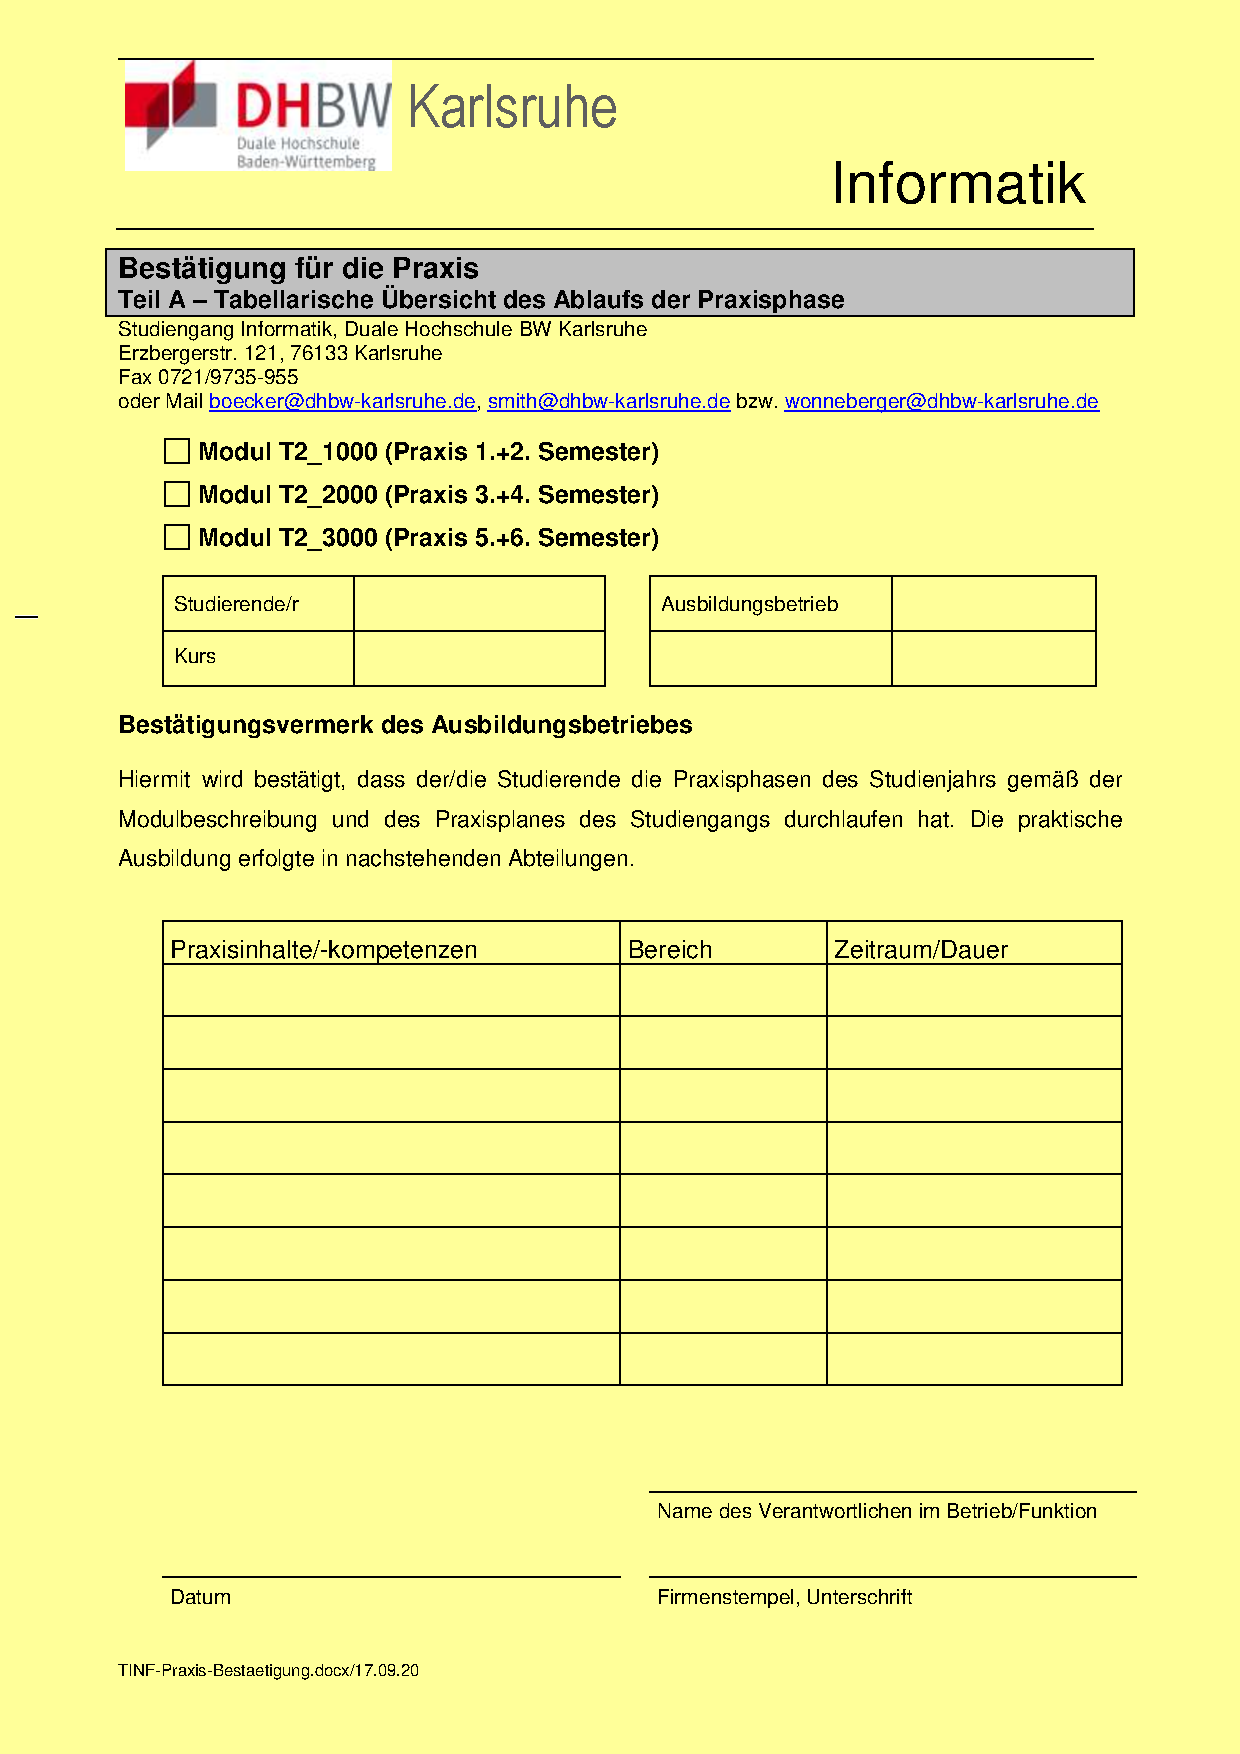
\includepdf[fitpaper=true, pages=1]{./zfiles/Dokumente/Teil-A}
		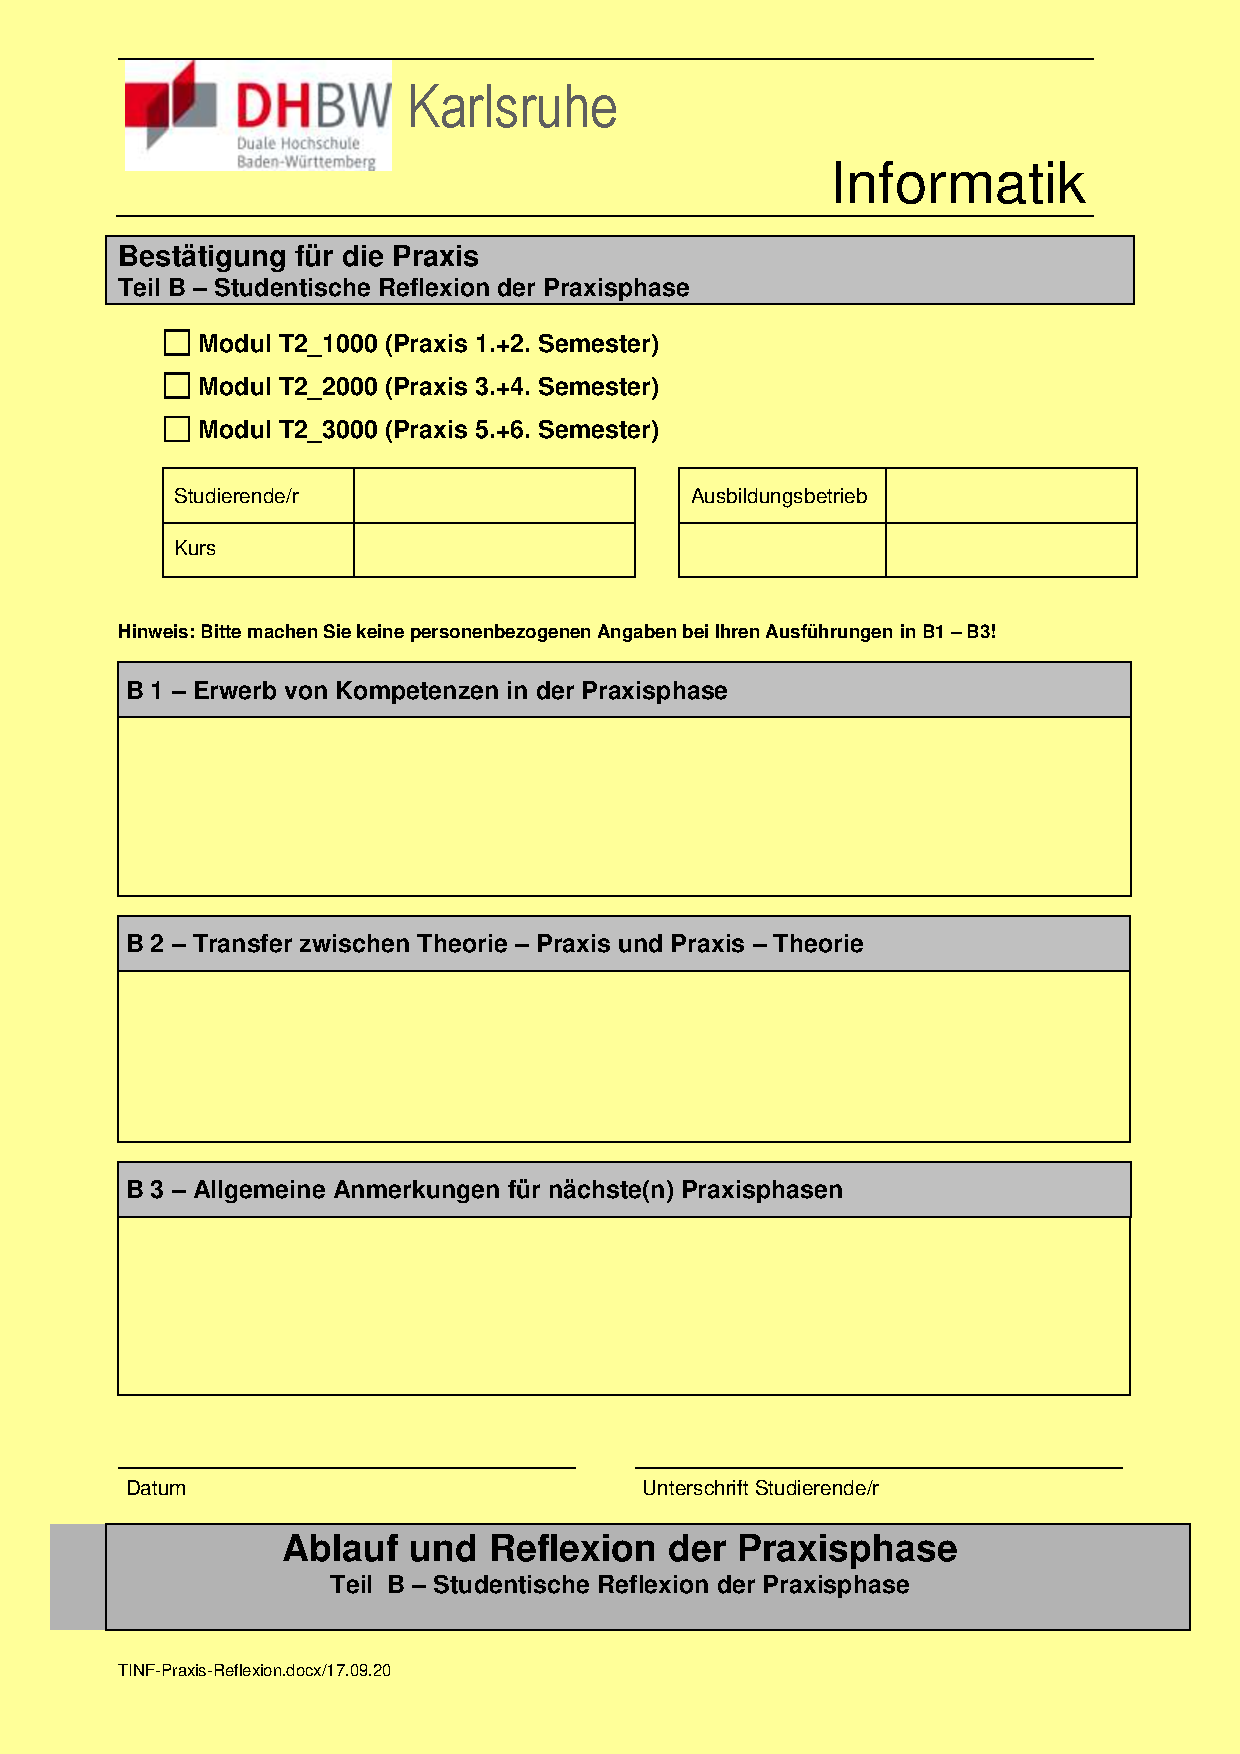
\includepdf[fitpaper=true, pages=1]{./zfiles/Dokumente/Teil-B}
		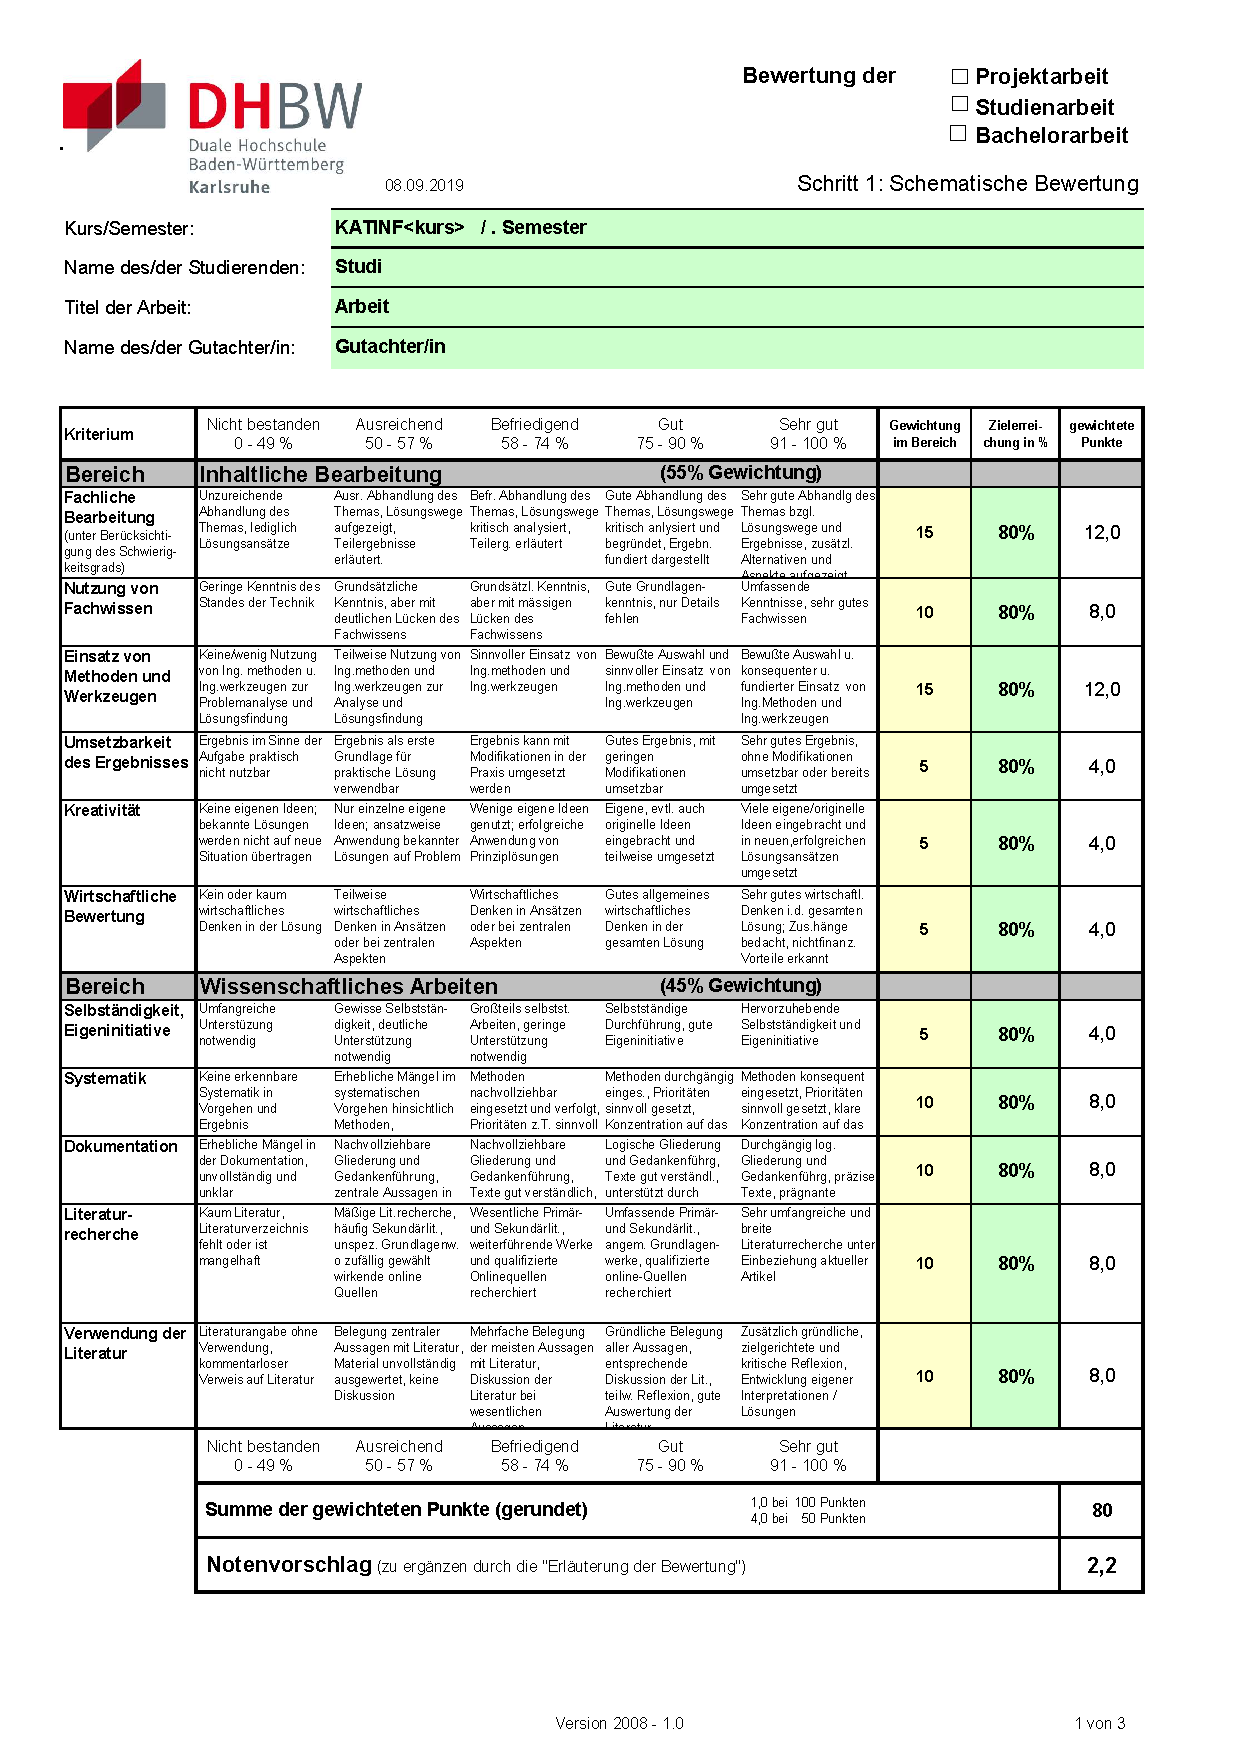
\includepdf[fitpaper=true, pages=1-3]{./zfiles/Dokumente/Bewertung}
	}{} 
	
	\ifthenelse{\boolean{DEBUG}}{}{\cleardoublepage}
\end{document}